\documentclass[12pt,a4paper]{article}
\usepackage {amsmath,amsthm}
\usepackage{geometry}
\usepackage{titlesec}
 \geometry{a4paper, total={170mm,257mm}, left=20mm, right=20mm, top=25mm, bottom=25mm}
\usepackage{sectsty}
\usepackage{natbib}
\bibliographystyle{econ}
\usepackage[hidelinks]{hyperref}
\usepackage{multirow}
\usepackage{makecell}
\usepackage{adjustbox}
%\usepackage{ulem}
\usepackage{threeparttable}
%\usepackage{prettyref}

%\usepackage[colorlinks=true, urlcolor=Blue]{hyperref}
%\usepackage{titling}
\sectionfont{\fontsize{14}{15}\selectfont}
\subsectionfont{\fontsize{13}{15}\selectfont}

\titleformat*{\section}{\LARGE\bfseries}
\titleformat*{\subsection}{\Large\bfseries}


\usepackage{caption}
\captionsetup{belowskip=0pt,aboveskip=6pt}

\makeatletter
\setlength{\@fptop}{0pt}
\makeatother

\makeatletter
\newcommand*\exInput[1]{\@@input#1 }
\makeatother


\usepackage[dvipsnames]{xcolor}

\newcommand{\link}[1]{{\color{blue}\href{#1}{#1}}}

%TRACKING TOOL FOR ARYA: 
\newcommand{\agt}[1]{{\color{OliveGreen}#1}}
\newcommand{\agst}[1]{{\color{OliveGreen}\sout{#1}}}

%TRACKING TOOL FOR ALEX: 
\newcommand{\aut}[1]{{\color{Red}#1}}
\newcommand{\aust}[1]{{\color{Red}\sout{#1}}}

%TRACKING TOOL FOR Peter: 
\newcommand{\pmt}[1]{{\color{Blue}#1}}
\newcommand{\pmst}[1]{{\color{Blue}\sout{#1}}}


%\usepackage{cite}
\usepackage{booktabs}
\usepackage{float}
\usepackage{setspace}
\usepackage{placeins}
\usepackage[list=true]{subcaption}
\captionsetup[sub]{font=footnotesize}

\usepackage{graphicx}


\newtheorem{theorem}{Proposition}
\newtheorem{hypothesis}{Hypothesis}
	\def\hypothesisautorefname{Hypothesis}
\newtheorem{result}{Result}
	\def\resultautorefname{Result}
\def\sym#1{\ifmmode^{#1}\else\(^{#1}\)\fi}


\title{\Large Willingness to Pay for Signals of Rare Events\\}
\author{\large Arya Gaduh, Peter McGee, Alexander Ugarov*}
\begin{document}
\maketitle
\onehalfspacing
\begin{abstract}{Designing multiple kinds of signals involves trade-offs between false-positive and false-negative costs. We conduct a laboratory experiment to evaluate preferences over these trade-offs in a controlled environment. We find that the choices significantly diverge from the predictions of the model with a risk-neutral decision-maker as well as from some predictions of expected utility frameworks. Relative to a risk neutral decision-maker, willingness-to-pay overreacts to false-negative rates for low priors, but underreacts for high priors. Subjects' preferences demonstrate a reverse bias for false-positive rates. This causes overpaying for signals with positive FP rates when the prior is low, and overpaying for all priors for low-quality signals with positive FP and FN rates. We find that this pattern is not consistent with the EU framework, but most consistent with a decision-making heuristic in which subjects do not differentiate between false-positive and false-negative rates when choosing signals.}


\vspace{10pt}
\begin{singlespace}
\noindent {\footnotesize{}JEL Classification: C91, D81, D84, D91}{\footnotesize \par}

\noindent {\footnotesize{}Keywords: alarms, value of information, information economics, information design, medical tests}{\thispagestyle{empty}}
\end{singlespace}
\end{abstract}

\vspace{180pt}
\newpage
\normalsize

\section{Introduction}

The 2010 gas blowout on Deep Horizon oil rig has killed 11 workers and caused one of the largest oil spills in history. The death toll was possibly aggravated by switching off a general safety alarm because its sirens interfered with workers' sleep.\footnote{https://www.nytimes.com/2010/07/24/us/24hearings.html} This illustrates the trade-off between false-positive and false-negative test results with false-positive rates leading to higher false alarm costs and false-negative resulting in missed events. 

Many real-life situations involve choosing binary tests to discover and prevent a negative outcome. Most binary tests transform continuous signals about the likelihood of an adverse state into simple yes/no prediction. This transformation relies on choosing a threshold for positive classification. Holding a continuous signal constant, a decrease in probability of no alarm in an adverse state (false-negative rate) corresponds to an increase in probability of alarm in a non-adverse state (false-positive rate). This trade-off motivates multiple discussions in medical diagnostics, alarm systems and extreme weather alerts. Despite ubiquity of binary alarms, there is little empirical evidence on how users evaluate alarms with different false-positive and false-negative rates. 

In order to understand preferences over these trade-offs, we study the demand for information in the framework with a potential protection action. The subject, first, receives a signal about the probability of an adverse event. Then she decides to protect or not. This environment describes several practically important scenarios including extreme weather alerts, medical testing and safety alarms. 

We find that the value of information in our setup weakly correlates with the willingness-to-pay. First, subjects on average underreact to quality of the signal, resulting in overpaying for low-quality signal and underpaying for high-quaity signals. Second, subjects tend to overreact to false-negative rates when the prior probability is low and overreact to false-positive positive rates when priors are high. We show that this pattern is most consistent with failure to estimate the effect of frequencies of false-positive and false-negative outcomes on the costs of using the signal. \citep{xu_revealed_2022} similarly finds that individuals do not properly account for priors and often choose tests not affecting optimal decisions even when more useful tests are available.

Our work is one of a few experimental studies measuring demand for information used for decision-making (instrumental information). Previous experimental studies studies the demand for signals in the prediction game in which subjects have to choose an optimal state under uncertainty. The field experiment conducted by \citep{hoffman_how_2016} finds that the demand for information increases with initial uncertainty, but decreases with the signal's accuracy. However, the decrease in accuracy is more modest than expected for a Bayesian decision-maker resulting in subjects underpaying for high-quality signals. The laboratory experiment of \citet{ambuehl_belief_2018} finds that subjects tend to underreact to the accuracy of the binary signal about state of the world, but put a premium on completely certain signals. The paper of \citet{xu_revealed_2022} also employs a prediction game setup to measure information preferences but varies priors on top of signal characteristics. She finds that many subjects choose non-instrumental over instrumental signals which is most consistent with failures of contingent reasoning on future value of information.

Our setup differs in two important aspects from \citep*{ambuehl_belief_2018, xu_revealed_2022}, because we study alerts and not prediction tasks. The subject faces a costly protection decision and not a prediction decision, resulting in three distinct payoffs: full payoff, full payoff minus protection costs and full payoff minus losses. It means that risk preferences affect the value of information and can change sensitivities to false-positive and false-negative rates. Our findings however are similar to prediction game findings. Consistent with \citet{ambuehl_belief_2018} we also find that subjects overvalue inaccurate signals, but we do not find a premium for certain signals.  And similar to \citet{xu_revealed_2022} we find that subjects commit reasoning errors leading to lower correlation between preferences and signal's usefulness in terms of cost reduction.

Due to its applicability for studying preferences over expectations, there is a larger stream of literature on the demand for non-instrumental information. \citet{eliaz_paying_2010} find that subjects are willing to pay for signals even when these signals are excessive for making optimal choices. Their design involves subjects choosing between two boxes with one box containing a prize of \$20. Most subjects pay just to know the probability of finding \$20 in box A even if this box is more likely to contain a prize in all the possible states. This finding is inconsistent with expected utility maximization but indicates instead having preferences for certainty before making choices.  Similar to this paper, \citet{masatlioglu_intrinsic_2017} also study preferences over information structures differing in false-positive and false-negative rates but their setup allows for a larger role of expectations. They find that for a positive potential outcome, most subjects prefer facing high false-negative rates rather than high false-positive rates. In other words, they tolerate uncertainty after negative signals better than uncertainty after positive signals. These preferences are salient: subjects require an average payment of 18-35 cents to switch to their least preferred information structure.

There is some mixed evidence that people update beliefs differently when these beliefs are ego-relevant or concern future gains and losses. \citet{eil_good_2011} find asymmetry in updating ego-relevant beliefs such as beauty and IQ. Subjects update more after receiving positive signals and do not update enough after negative signals. Additionally, subjects with high posterior ego-relevant beliefs are willing to pay to receive a more precise signals, but require a compensation for learning when their beliefs are low. In contrast, \citet{coutts_good_2019} does not find any updating asymmetry with respect to either ego-relevant beliefs or beliefs about future payoffs. 

Our paper is the first to measure value of information in the experimental setting of diagnostic tests or alarms. Previous work studies the use of alarms in context of medical testing, medical monitoring, safety alarms and extreme weather. Early literature on decision-making of medical professionals finds that doctors suffer from multiple biases when ordering testing, including  inaccurate posterior probability estimation due to availability heuristics, hindsight bias and regret \citep{bornstein_rationality_2001}. \citet{gigerenzer_helping_2007} find that most mammologists tend to overestimate the probability of cancer based on a positive result. Providing practitioners with natural frequencies instead of probabilities tends to reduce this bias.  

Patients' willingness-to-pay for medical tests is large and sensitive to test accuracy \citep{liang_acceptability_2003, howard_does_2009, neumann_willingness--pay_2012}. But test preferences also exhibit several abnormalities. First, users are willing to pay for tests having little or zero diagnostic value \citep{schwartz_enthusiasm_2004, neumann_willingness--pay_2012}. For example, \citet{schwartz_enthusiasm_2004} find that 73\% of Americans in their survey prefer a free full-body CT scan versus one thousand USD cash. However, medical professional do not recommend full-body CT scans for healthy people due to extreme likelihood of false-positive findings. Second, the framing of test accuracy seems to matter a lot. \citet{howard_does_2009} conduct a discrete-choice experiment to measure willingness-to-pay for the colorectal cancer screening. Their subjects agree to get 23 unnecessary colonoscopies in order to find one additional true cancer, but only 10.4 for reducing the number of cancers missed by one even though these descriptions are equivalent. Surprisingly, the perceived risk of cancer (prior) did not significantly affect the WTP in their study.

Our work also relates to the vast literature on demand for insurance and protection. Similar to our findings, several studies observe that the demand for insurance goes up after the recent experience with low probability events. Field evidence indicates that people under-insure with respect to rare natural disasters \citep{friedl_insurance_2014}. \citet{laury_insurance_2009} find no under-insurance for low-probability events in the laboratory setting. One offered explanation \citep{volkman-wise_representativeness_2015} is that subjects overweight recent evidence leading to under-insurance when there were no negative events in the recent past and to overinsurance after the fact. It is consistent with underweighting prior probabilities relative to more recent signals. 

The bias we are finding is similar to the base-rate and signal neglect phenomenons. Psychology researchers \citet{hammerton_case_1973} and \citet{kahneman_psychology_1973} first observed that subjects underweighted prior probabilities (base rates) when calculating posteriors. This phenomenon had received the name of \textit{base-rate neglect}. Multiple studies in economics then confirmed \citep*{grether_testing_1992, holt_update_2009} this phenomenon in incentivized laboratory experiments. Most of these studies find that subjects also underweight signals on top of priors.  We observe both phenomenons in responses to our belief elicitation task, but the calculation of signals' values differs substantially from the calculation of posterior probabilities. While the calculation of posterior probabilities would require using a Bayes formula, signal's value depends only on products of prior probabilities. However, we observe that subjects underestimate the effect of priors compared to theoretical predictions for an expected-utility decision-maker.

As we use use a strategic approach to elicit both beliefs and hypothetical choices, our subjects has to participate in contingent reasoning. \citet{aina_contingent_2023} recently find that contingent reasoning increases bias in belief elicitation. Belief biases and protection decisions can be reduces by eliciting responses after presenting a signal. Decisions to acquire information however fundamentally rely on thinking through contingencies.

\vspace{20pt}
\section{Model}
\paragraph{Environment.} Consider an agent's purchase of threat assessment information. Let $\omega \in \{0,1\}$ denote the state of world, where 1 corresponds to an adverse event happening with probability $\pi$. Without a protective action, the agent has a lower utility in the adverse state. Protective action $a\in\{0,1\}$ completely eliminates losses, so that the bad outcome happens only when $\omega(1-a)=1$.

Agent's preferences are described by the utility function which depends on income $Y$, protective action $a$, and the protective outcome $\omega(1-a)$. Taking protective action reduces income by $c>0$. Utility is separable in wealth, protection cost $c>0$ and the potential loss $L>c$ in the adverse state if not protected:
\begin{equation}
U=U(Y,a,\omega(1-a))=u(Y-ac-\omega(1-a)L)
\end{equation}

The agent can purchase a binary signal $s\in\{0,1\}$ about the state of the world before making a decision. Let $P_{ij}\equiv P(s=i|\omega=j)$ be the probability of a signal $s$ taking value $i$ conditional on the state of the world being $j$.  After receiving the signal, the agent updates her belief on the likelihood of the bad state to $\mu(s)$. Unless specified otherwise, we assume that she is Bayesian and hence her posterior belief equals:
\begin{equation}
\mu(s)= {\pi P_{s1} \over \pi P_{s1}+(1-\pi)P_{s0}}
\end{equation}

Without loss of generality, we also assume that a higher signal means a higher posterior probability of an adverse event $\mu(1)\geq\mu(0)$. Otherwise we can always re-label the signals.

\vspace{10pt}
\paragraph{Preferences.} If there is no signal, the agent protects if and only if it increases her expected utility:
\begin{equation}
EU_0=\max[u(Y-c),\pi u(Y-L)+(1-\pi) u(Y)]
\end{equation}
The signal can increase expected utility if the agent reacts differently to positive and negative signals. Under these assumptions, her expected utility with a signal is:
\begin{equation}
EU_s=\pi P_{11}u(Y-c)+\pi P_{01}u(Y-L)+(1-\pi)P_{10}u(Y-c)+(1-\pi)P_{00}u(Y)
\end{equation}

We consider the maximum amount $b$ which the agent is willing to pay for the signal. In our framework, $b$ is the price such that an agent is indifferent between paying $b$ to have the signal and not having a signal. Because the agent can always ignore a useless signal, the signal's value is bounded from below by zero. Hence it equals to the maximum between zero and the solution to the following equation:
\begin{equation}
\begin{split}
P(s=1)u(Y-b-c)+\pi P_{01}u(Y-b-L)+(1-\pi)P_{00}u(Y-b)=\\=\max[u(Y-c),\pi u(Y-L)+(1-\pi) u(Y)] 
\end{split}
\end{equation}

Here we use $P(s=1)\equiv \pi P_{11}+(1-\pi)P_{10}$ to denote the probability of a positive signal (alert). The left-hand side expression of this equation is a strictly decreasing function of $b$. Additionally, for $b\rightarrow \infty$ the left-hand side is smaller than the right-hand side. It implies that the equation (5) above has a at most one positive solution.

Obviously, a perfectly accurate signal always has positive value $b>0$ because the payoff distribution with the signal first-order stochastically dominates the distribution without the signal. 
%If the agent protects without a signal, a perfect signal reduces the protection costs and if she takes chances, then it reduces losses in the adverse outcome from $L$ to $c<L$.  
However, it is harder to determine the value of the imperfect signal without imposing more restrictions on preferences as it requires weighing $u(Y-L)$ against $u(Y-c)$.


\paragraph{Risk-neutral agent.} If the agent is risk-neutral, the expression above collapses to:
$$b+P(s=1)c+\pi P_{01}L=\min[c,\pi L]$$

The signal's value is just:
\begin{equation}
b=\max[0,\min[c,\pi L]-P(s=1)c-\pi P_{01}L]
\end{equation}

We can express the WTP $b$ as a function of priors, false-positive (FP), and false-negative rates (FN) denoted correspondingly as $P_{10}$ and $P_{01}$. This is the equation we use in our empirical work:
\begin{equation}
b=\max[0,\min[c,\pi L]-\pi (1-P_{01})c-(1-\pi)P_{10}c-\pi P_{01}L]
\end{equation}\label{eq:rnWTP}

For a useful signal ($b>0$) the sensitivity of WTP $b$ with respect to FP $P_{10}$ and FN $P_{01}$ rates is given by:
\begin{equation}
{db\over dP_{10}}=-(1-\pi)c
\end{equation}

\begin{equation}
{db\over dP_{01}}=-\pi(L-c)
\end{equation}
\vspace{10pt}

Both FP and FN rates decrease the (positive) signal's value. The effect is proportional to the adverse state probability for the false-negative rate and to the non-adverse state probability for the false-positive rates.

\paragraph{Risk Aversion Effects.} In a more general expected utility framework, risk aversion can both increase and decrease the signal's value. More specifically, risk aversion decreases the value when the protection costs are low: 

\begin{theorem}
 If protection costs are low $c<\pi L$, then a strictly risk-averse decision-maker pays less than a risk-neutral one.
\end{theorem} 
\begin{proof}
See the Appendix.
\end{proof}

%\normalsize
It is harder to make definite statements for lower risks or higher protection costs. For example, risk aversion increases the value of a perfect signal as long as a risk-averse decision-maker still chooses to not protect without a signal. This follows from the standard argument of increasing demand for insurance with risk aversion and the fact that the protection problem with a perfect signal is isomorphic to the insurance problem with deductible $c$. 
Next, we study the effect of false-positive and false-negative rates on the signal's value $b$. Assuming a differentiable utility function $u()$ we use implicit differentiation to derive sensitivities of WTP $b$ to false-positive and false-negative rates:

$${db\over dP_{10}}=-{(1-\pi)(u(Y-b)-u(Y-c-b))\over D(\pi, P_{01}, P_{10}, b)}$$
$${db\over dP_{01}}=-{\pi(u(Y-c-b)-u(Y-L-b))\over D(\pi, P_{01}, P_{10}, b)}$$

With the denominator equal to the expected marginal utility:
$$D(\pi, P_{01}, P_{10}, b)\equiv P(S=1)u'(Y-c-b)+\pi P_{01}u'(Y-L-b)+$$
$$+(1-\pi)P_{00}u'(Y-b)=E[MU]>0$$

It is clear that the signal's value decreases with FP and FN rates ${db\over dP_{10}},{db\over dP_{01}}<0$. We can also say a bit more about the sensitivity to FN rates:
\begin{theorem}
Risk-averse and imprudent decision-maker has higher sensitivity to FN rates as compared to a risk-neutral one.
\end{theorem}\label{thm:riskAverse}  
%\small
\begin{proof}
See the Appendix.
\end{proof}
%\normalsize

However, risk aversion can both increase and decrease subject's sensitivity to FP rates depending on the utility function's curvature and the signal's characteristics. Intuitively, an expected marginal utility of a strongly risk-averse subject with a bad signal can be lower than the average slope of the utility function between ($Y-c-b$) and ($Y-b$) which reduces sensitivity to FP rates. It can also be higher if either the signal is good or the curvature is small. We can only say that it is very likely that for low protection costs and small priors $\pi$ (leading to no automatic blind protection) the ratio of sensitivities to FP rates over FN rates should be lower for risk-averse subjects. 

\begin{theorem}
For low protection costs $c$ and small risks $\pi$, risk aversion lowers relative sensitivity to FP rates. 
\end{theorem}\label{thm:riskAverse2}  

\begin{proof}
See the Appendix.
\end{proof}
%\normalsize


%\vspace{10pt}
\noindent Based on the analysis of the model we propose two hypotheses to test in the experiment:
%\begin{enumerate}
%\item 
\textbf{\textit{Hypothesis 1}: Subjects' WTPs for signals equal to their value for risk-neutral agents.} The risk-neutral model predicts an easily calculated value for the willingness-to-pay $b$ for the signal. Depending on signal characteristics and risk preferences, agents can pay more or less than the risk-neutral benchmark.

 
%\item 
\textbf{\textit{Hypothesis 2}: Subjects' preferences demonstrate equal sensitivity to costs generated by false-positive and false-negative events.} The model of a risk-neutral agent suggests that they should. Our derivations above indicate that the relative weight of false-negative costs can be either below or above one depending only on risk preferences.
%\end{enumerate}




\vspace{20pt}

\section{Experimental Design}

The experiment was conducted in the Behavioral Business Research Lab (BBRL) at the University of Arkansas between October and November 2021.  A total of 105 subjects participated in an individual decision task implemented using Qualtrics.  On average, including a \$5 show-up fee, subjects earned \$26 for a session lasting around 45 minutes. 
%84 percent of the subjects were university students and 41 percent were male.  About 60 percent of the subjects had taken at least one statistics course. 
 
In addition to the show-up fee, subjects were endowed with \$25 that they could potentially lose in the experiment, an outcome which was determined by a series of decisions in four sets of tasks played in the following order: (i) Blind Protection; (ii) Informed Protection; (iii) Belief Elicitation; and (iv) Willingness to Pay Elicitation. Subjects took a quiz of understanding prior to each task; the correct answer and an explanation were provided if a subject answers a question incorrectly.\footnote{Incorrect answers in quiz for the Informed Protection section results in subjects facing additional questions. In our opinion, clear understanding of the Informed Protection task is essential for subsequent tasks, hence the added requirement.  These questions consist of XXX; complete details are in the appendix.} Each task consisted of 6 rounds, resulting in 24 total rounds. At the end of the experiment, one of these 24 rounds is is randomly selected as the payment round. The instructions can be found in the appendix.


\bigskip
\noindent\textbf{Blind Protection (BP)}.\ \ \ Subjects must decide whether to protect against an adverse event: a random draw of a black ball.  Subjects know the prior probability that a black ball is drawn. Protection costs \$5. A subject who draws a black ball will lose nothing if they chose to protect and \$20 if they did not. The prior probability of drawing a black ball across the 6 rounds is denoted as $p \in \{0.05,0.10,...,0.3\}$. The order was common for all the subjects and started at the lowest probability. Subjects did not receive feedback on the realization of the decision.

\bigskip
\noindent\textbf{Informed Protection (IP)}.\ \ \ Similar to the BP task, subjects must make a protection decision given the prior probability of drawing a black ball. In addition to the prior, subjects also receive a signal with varying degrees of inaccuracy. Following \citet{coutts_good_2019}, we use a group of hinting gremlins to convey signal accuracy: a gremlin, randomly drawn from a group, gives out the signal. The gremlin is one of three types: (i) honest; (ii) ``black-swamp'' who always says that the ball is black; and (iii) ``white-swamp'' who always says that the ball is white. Figure~\ref{fig:Gremlins} illustrates how the different gremlin types were presented to the subjects. The composition of the group of gremlins determines signal accuracy: a higher share of black(white)-swamp gremlins produces a signal with higher FP (FN) rate. Subjects know the group composition, but do not know which gremlin provides the hint. We vary the proportion of prior probability of drawing a black ball and the composition of gremlins across rounds.  

\begin{figure}[H]
\centering
\caption{Signals Presentation} \label{fig:Gremlins}
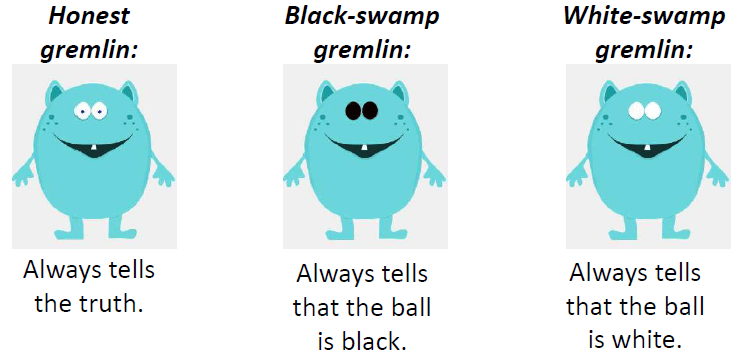
\includegraphics[width=0.6\textwidth]{Graphs/gremlins1.png}
\end{figure}


\bigskip
\noindent\textbf{Belief Elicitation (BE)}.\ \ \ 
%We use the BE task to elicit subjects' beliefs about the likelihood of an adverse event and an adverse signal conditional on prior and signal characteristics in an incentive-compatible way. Similar to 
As in the IP task, subjects know the prior probability of drawing a black ball and the composition of the group of gremlin providing hints. Instead of making a protection decision, however, subjects are asked to estimate the probability that: (i) the ball is black when the gremlin says that it is white; (ii) the ball is black when the gremlin says that it is black. 

To elicit incentive-compatible responses, we follow the stochastic version of the Becker-DeGroot-Marshak mechanism developed by \citet{grether_testing_1992} and \citet{holt_update_2009} \aut{but stated equivalently in terms of losses rather than gains to match the description of other tasks. Subjects submit their beliefs about the probability of the event $\mu \in [0,1]$. If this belief is above some uniform random number $r\in[0,1]$, they bear a loss of 20 USD only if the event happens, i.e., the ball is black. If the random number $r$ is above their reported belief, then their payoff is determined by an independent lottery which loses 20 with probability $r$ and 0 otherwise.\footnote{The benefit of this mechanism versus other probability elicitation mechanisms (e.g., quadratic scoring) is that reporting truthfully is a dominant strategy regardless of risk preferences \citep{karni_mechanism_2009-1}. The only requirements a subject must satisfy are probabilistic sophistication and dominance: they rank lotteries based on their probabilities only and prefer higher probabilities of higher payoffs.} Motivated by \citet{danz_belief_2020} who find that providing a detailed explanation of payoffs can lower trustfull reporting, we instead provide our subjects with the explanation that reporting true belief $\mu$ maximizes their payoffs, and give an example of payoff calculation under different reporting strategies.}

\bigskip
\noindent\textbf{Willingness to Pay Elicitation (WTPE)}.\ \ \ The WTPE task measures a subject's willingness to pay (WTP) for signals. As before, subjects know the prior probability of drawing a black ball and the composition of the group of gremlin providing hints.  Unlike the IP task, subjects do not automatically receive a hint, instead they provide their WTP for a hint by choosing a value $\in{\$0,\$5}$ in\$0.50 increments. The elicitation is incentive compatible: if a WTPE round is selected as the payment round, a random price of a hint will be drawn. If that price exceeded the subject's WTP, they will play a BP round, otherwise the subject pays their WTP and plays an IP round.  

\vspace{10pt} 

After the WTPE task, subjects answered a few demographic questions.\footnote{\aut{These were the questions on subjects' gender, age, and experience of taking statistics classes.}} After the demographic questions, the algorithm randomly selectst the payment task and the payment round to calculate the subject's payoff. 
%, as well as the gremlin groupings (along with the associated false positive and false positive rates) that we used for the different tasks.

\aut{With the exception of the first task (Blind Protection), other tasks involve subjects going through two different priors and three types of signals. The order is such that subjects go consecutively over all three signals starting from the honest one for each prior. The order of priors and signals stays constant for each subjects across tasks, but can vary between subjects. Table~\ref{tab:treatments} summarizes our treatments.}

%%%%%%%%%%%%%%%%%%%%%%%%%%%%%%%%%%%%%%%%%%%%%%%%%%%%%%%%%%%%%%%%%%%%%%%%%%%%%%%%%%%%%%%%%%%%%%%%%%%%%%%%
\begin{table}[h!]
\caption{List of Treatments} \label{tab:treatments}
\begin{tabular}{l*{6}{c}}
\hline\hline
 & \multicolumn{3}{c} {Gremlins composition} & & \\
Prop. of black balls ($p$) & Honest & Black-eyed &White-eyed & FP rate &  FN rate\\
\hline
0.1, 0.2, 0.3, 0.5         &    2 & 0  &  0 & 0 & 0\\

0.1, 0.2, 0.3, 0.5         &    3 & 1  &  0 & 0.33 & 0  \\

0.1, 0.2, 0.3, 0.5          &    3 & 0  &  1 & 0 & 0.33 \\

0.1, 0.2, 0.3, 0.5           &    3 & 1  & 1 & 0.33 & 0.33\\

0.1, 0.2, 0.3, 0.5         &    5 & 1  & 0 & 0.2 & 0\\
0.1, 0.2, 0.3, 0.5         &    5 & 0  & 1 & 0 & 0.2    \\
0.1, 0.2, 0.3, 0.5         &    5 & 1 & 1  & 0.2 & 0.2  \\
\hline\hline
\end{tabular}


\end{table}

%%%%%%%%%%%%%%%%%%%%%%%%%%%%%%%%%%%%%%%%%%%%%%%%%%%%%%%%%%%%%%%%%%%%%%%%%%%%%%%%%%%%%%%%%%%%%%%%%%%%%%%%

 


\vspace{20pt}
\section{Subject Decisions By Task}\label{sec:sanity}

Decisions in the Blind Protection (BP), Informed Protection (IP), and Belief Elicitation (BE) tasks measure factors determining WTP in our model. Protection choices in the BP task reveals subjects' risk preferences with known probabilities. Choices in the IP task demonstrate how subjects use signals given their characteristics. Finally, the BE task provides insight into subjects' beliefs for given signals.  We provide details below, but, on average, subjects appear to understand these tasks reasonably well.
%Some of these tasks can be quite challenging. However, we show below that 

\subsection{Blind Protection}

Figure~\ref{fig:ProtResponse} plots the likelihood of choosing to protect against the posterior probability of a drawing a black ball for the BP task, where the posterior is equivalent to the prior, and in the IP task. On aggregate in the BP task, subjects' likelihood of protecting increases in the probability of a negative outcome: only 13\% subjects protect when the probability of a black ball is 10\% in contrast to 70\% protecting when the probability is 30\%. 

At the individual level, BP responses indicate significant heterogeneity in risk preferences. For approximately 70\% of subjects (72/105), protection action increases monotonically in probability. The remaining 30\% make at least one switch from protecting to not protecting and back, which is inconsistent with EU maximization. Among these switchers, however, 83\% (24/39) skip only a single increment of the presented probability scale, suggesting an inattention error.\footnote{For comparison, Holt and Laury (2002) for a similar instrument find that 28 of 212 subjects (13\%) switched back to a low-risk option with an increasing likelihood of high payoffs in a risky option at least once when decisions were presented in increasing order, which they are not here.} 

Risk-neutral agents who maximize their expected utility should start protecting when the prior exceeds 0.25, i.e., at the ratio of the protection cost to the potential loss = \$5/\$20). Many of our subjects start protecting at lower priors, indicating strict risk aversion.\footnote{As a reference, switching at the probability 0.1 corresponds to a CRRA risk aversion $\theta=2$, while switching at 0.2 corresponds to $\theta=0.57$.}  A smaller group of subjects makes choices consistent with risk loving by protecting at a probability of 0.3 or never protecting. 

\subsection{Informed Protection}

Recall that, in the IP task, subjects receive a signal about the color of the ball in addition to the prior. 
Figure~\ref{fig:ProtResponse} shows that protection actions are increasing in the posteriors, though roughly 28\% of subjects break monotonicity in their protection responses with respect to posterior probabilities --- approximately the percentage of non-monotonic responses in the BP task.\footnote{That is, subjects do not protect for some treatments with posterior probability $P$ while protecting for a posterior probability $P'<P$.}  At the individual level, we also find that the total number of times subjects protect in the BP task significantly correlates with their likelihood to protect in the IP task conditional on posteriors, but this explains only a very small part ($<$1\%) of variation in the IP decisions.\footnote{We use a linear probability model to estimate this relationship, and while the coefficient on the total number of protection choices is significant at the 1\% level, the $R^2$ only increases from 0.295 to 0.3.} 


%%%%%%%%%%%%%%%%%%%%%%%%%%%%%%%%%%%%%%%%%%%%%%%%%%%%%%%%%%%%%%%%%%%%%%%%%%%%%%%%%%%%%%%%%%%%%%%%%%%%%%%%%%%%%%%%%%%

\begin{figure}[H]
\centering
\caption{Average Protection Response} \label{fig:ProtResponse}
\begin{subfigure}[t]{.45\textwidth}
  \centering
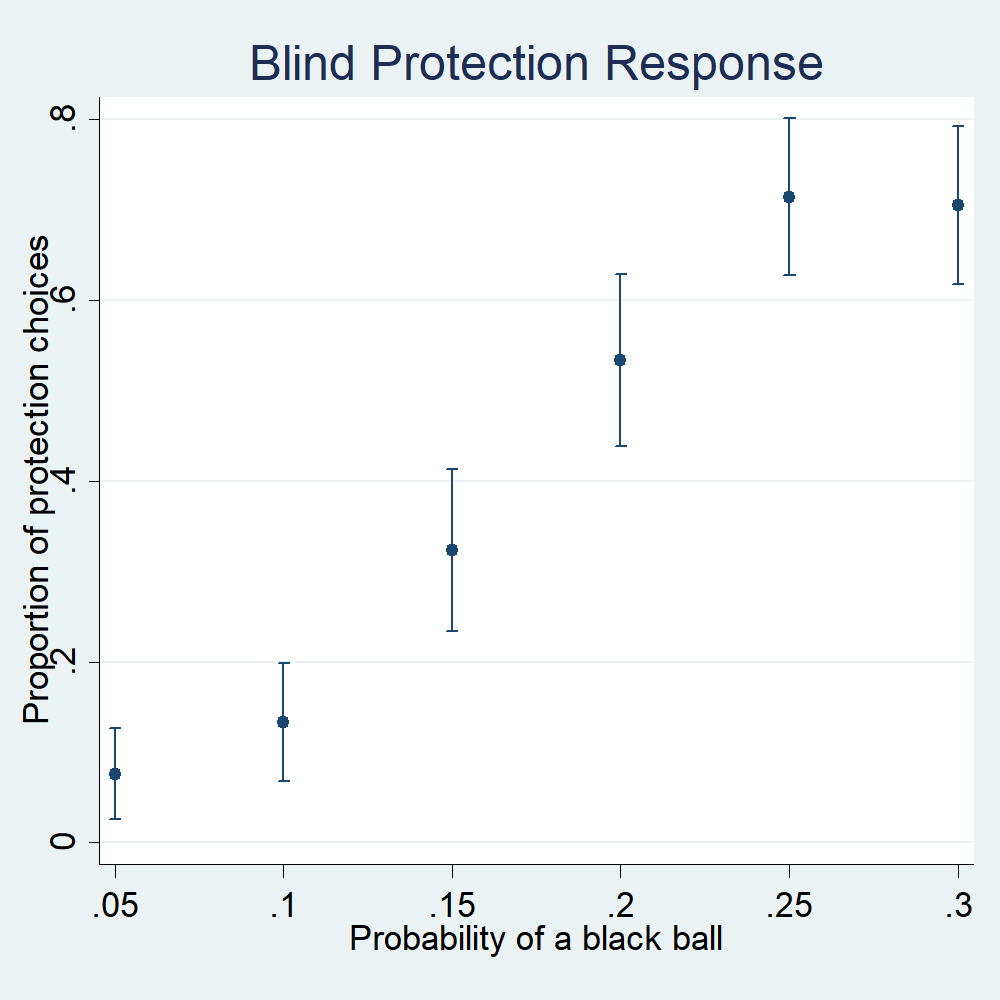
\includegraphics[width=\textwidth]{Graphs/blind_prot_sta.png}
\caption{The bars show 95\% confidence intervals for the mean proportion of subjects choosing protection at each prior probability.}
\end{subfigure}
\begin{subfigure}[t]{.45\textwidth}
  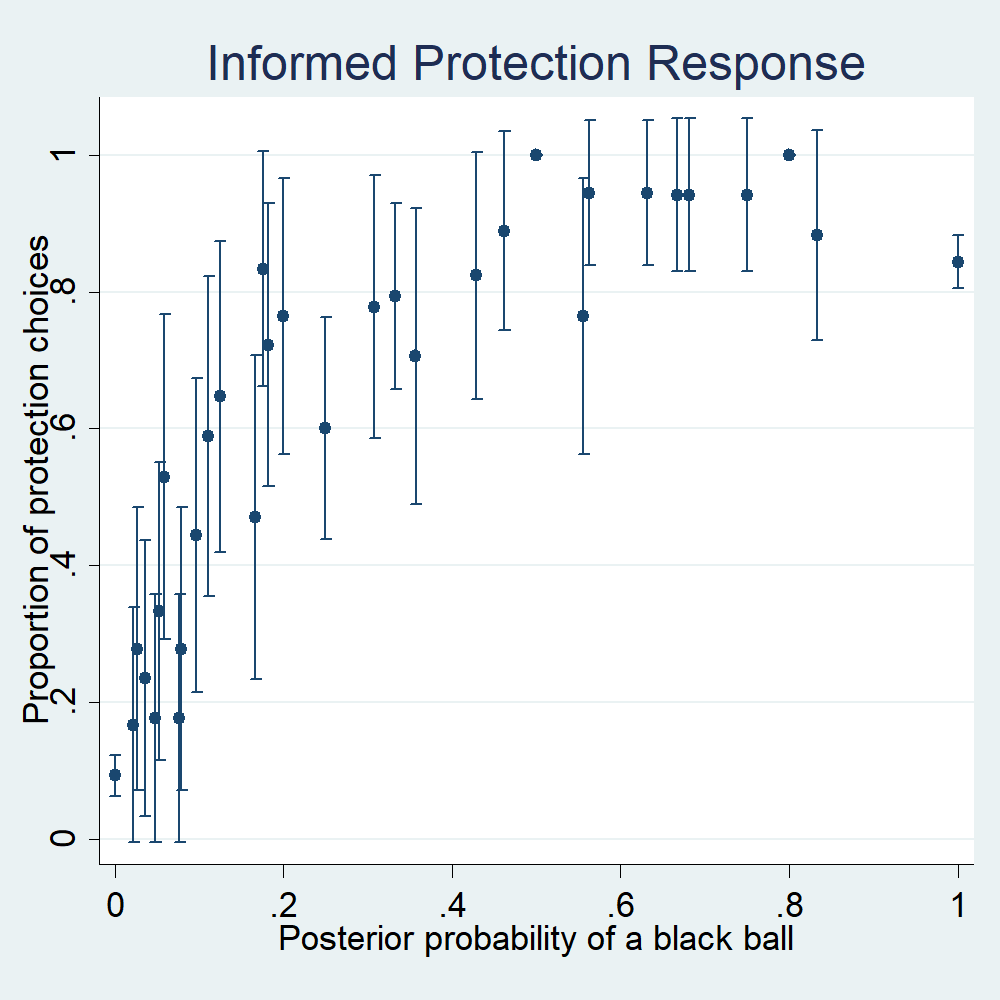
\includegraphics[width=\textwidth]{Graphs/ip_response.png}
\caption{The bars show 95\% confidence intervals for the mean proportion of subjects choosing protection at each posterior probability.}
\end{subfigure}
%\begin{subfigure}[t]{.48\textwidth}
  %\centering
  %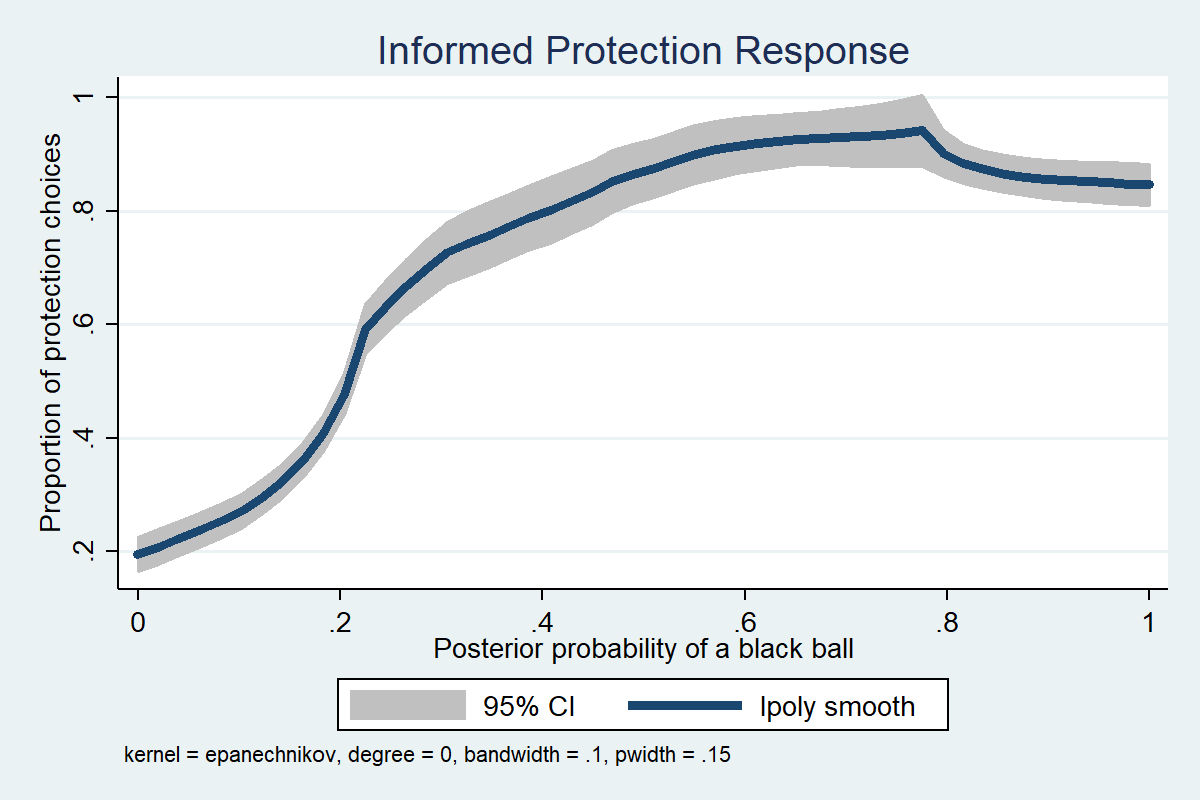
\includegraphics[width=\textwidth]{Graphs/ip_response_lpoly.png}
%
%\end{subfigure}
\end{figure}
%\pmt{Eventually we need to add notes to the figures}
%%%%%%%%%%%%%%%%%%%%%%%%%%%%%%%%%%%%%%%%%%%%%%%%%%%%%%%%%%%%%%%%%%%%%%%%%%%%%%%%%%%%%%%%%%%%%%%%%%%%%%%%%%%%%%%%%%%

Table~\ref{tab:nonparIP} presents the average protection decisions by signal characteristics. The first three columns summarize the signal characteristic information available to the subject. Column 4 shows the posterior probability of a black ball averaged across all the treatments within a group. Column 5 shows the subjects' share of empirical protection responses, next to the theoretical optimum for risk-neutral subjects in Column 6. Column 7 presents the $p$-value for a test of equality between empirical and theoretical protection responses.

We make three notable observations. First, regardless of false-positive (FP) and false-negative (FN) rates, black signals substantially increase the likelihood of protection.  Second, subjects' protection decisions deviate significantly from what is optimal for risk-neutral subjects in most treatments, as evidenced by column 7: subjects tend to overprotect when facing white signals (rows 1--4) and underprotect when facing black signals (rows 5--8), with the exceptions a black signal and positive FP rates where the statistical equality of columns 5 and 6 cannot be rejected (rows 7--8).

%\textbf{In light of BP decisions it is not surprising that subjects do not behave as risk-neutral agents, but some biases cannot be explained by the expected utility maximization for any degree of risk aversion.} 
Third, we find that some deviations cannot be explained by the expected utility maximization for any degree of risk aversion. For example, consider rows 1 and 3: even though an increase in the signal's FP rate does not change the posterior (because the signal is white), the protection rate increases by 6 percentage points (pp). Similarly, row 4 shows that when both FP and FN are positive, the protection rate increases to 56 percent --- even though the average (maximum) posterior probability for the signal characteristics is just 13 percent. As a benchmark, with no signal in the BP task, only 13~(32) percent of subjects choose to protect when the probability is 10~(15) percent. 

%%%%%%%%%%%%%%%%%%%%%%%%%%%%%%%%%%%%%%%%%%%%%%%%%%%%%%%%%%%%%%%%%%%%%%%%%%%%%%%%%%%%%%%%%%%%%

\begin{table}[H]\centering 
\caption{Average Protection by Signal Type} 
\label{tab:nonparIP}
\adjustbox{max width=\textwidth}{
	\begin{threeparttable}
	\begin{tabular}{cccccccc} \hline \hline
	\multirow{4}{6ex}{\centering \textbf{Row}}
			&\multicolumn{3}{c}{\centering \textbf{Signal Characteristics}} 
			& \multirow{3}{10ex}{\centering \textbf{Posterior}} & \multirow{3}{10ex}{\centering \textbf{Share Protect}} 
			& \multirow{3}{10ex}{\centering \textbf{Share Optimal}} 
			& \multirow{3}{13ex}{\centering \textbf{P-val $(H_0: (5)=(6))$}} \\ 
			\cmidrule(lr){2-4}
		&\multirow{2}{12ex}{\centering \textbf{Signal}} & \multirow{2}{12ex}{\centering \textbf{False Positive}} 
			& \multirow{2}{12ex}{\centering \textbf{False Negative}} 
		\\
		\\
		&(1) & (2) & (3) & (4) & (5) & (6) & (7) \\
		\hline
			(1)&White&No&No&0.000&0.067&0.000&0.000\\
(2)&White&No&Yes&0.100&0.333&0.000&0.000\\
(3)&White&Yes&No&0.000&0.130&0.000&0.000\\
(4)&White&Yes&Yes&0.131&0.564&0.121&0.000\\
(5)&Black&No&No&1.000&0.846&1.000&0.000\\
(6)&Black&No&Yes&1.000&0.841&1.000&0.000\\
(7)&Black&Yes&No&0.550&0.833&0.870&0.355\\
(8)&Black&Yes&Yes&0.483&0.886&0.871&0.685\\

			\\[-1em]
		\hline\hline 
	\end{tabular} 
	\begin{tablenotes}[flushleft]
			\item\leavevmode\kern-\scriptspace\kern-\labelsep \footnotesize \textit{Notes:} 
	\end{tablenotes}								
	\end{threeparttable}
	}
\end{table}



%\bigskip\noindent\textbf{Belief Elicitation.}\ \ \ 
\subsection{Belief Elicitation}
Subject decisions in the IP task capture the use of signals in protection decisions, but decisions reflect but risk preferences and (potentially erroneous) beliefs.  The BP task can be used to construct a measure of the former; the BE task to measure the latter.  


%%%%%%%%%%%%%%%%%%%%%%%%%%%%%%%%%%%%%%%%%%%%%%%%%%%%%%%%%%%%%%%%%%%%%%%%%%%%%%%%%%%%%%%%%%%%%%%%%%%%%%%%%%%%%%%%%%%

\begin{figure}[H]
	\centering
	\caption{Errors in Bayesian Updating} \label{fig:BeliefUpdate}
	\subcaptionbox{Error Distribution}{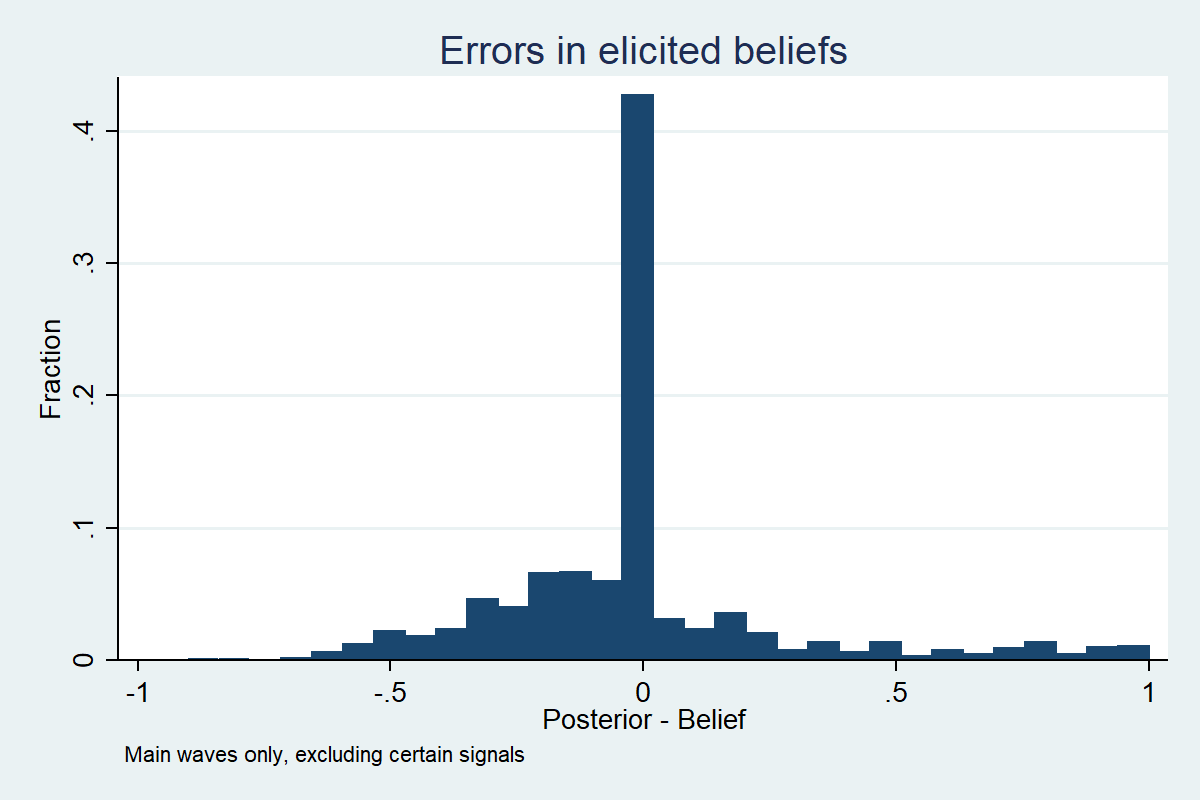
\includegraphics[width=.48\textwidth]{Graphs/hist_belief_error_s3.png}}
	\hfill
	\subcaptionbox{Error v. Posterior}{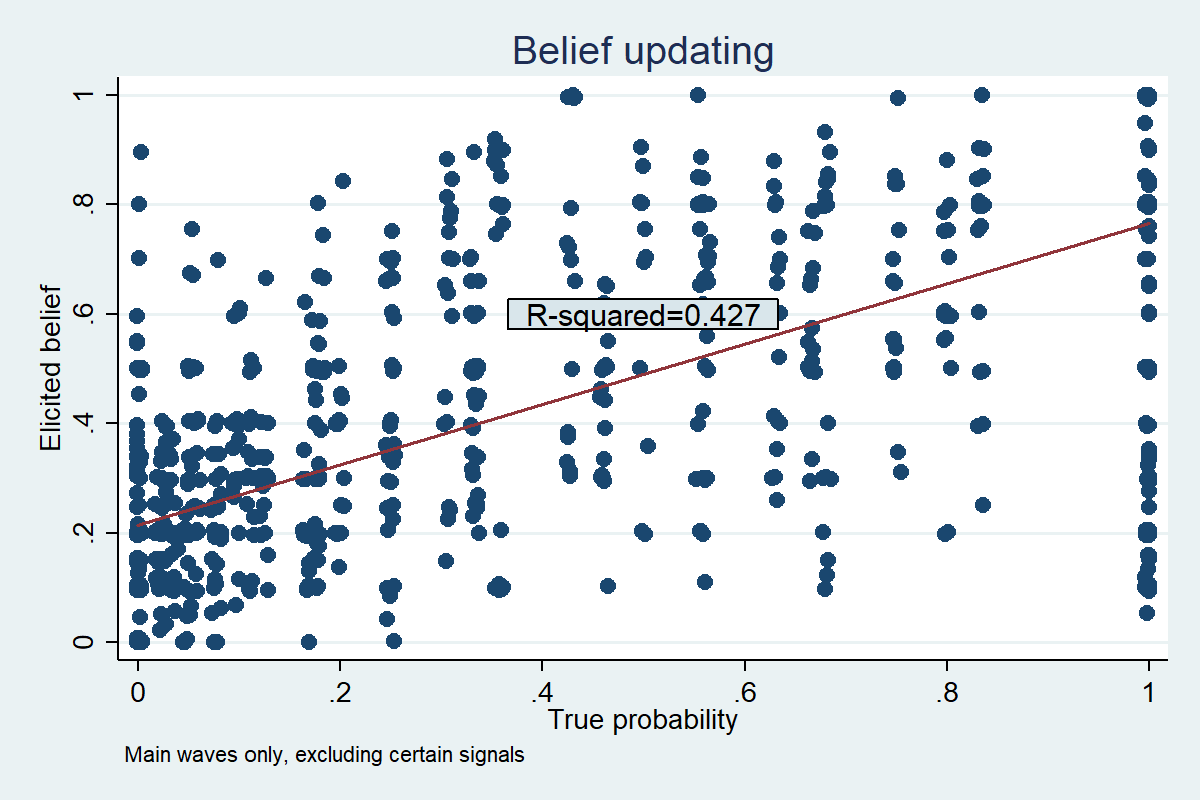
\includegraphics[width=.48\textwidth]{Graphs/updating_s3.png}}
	\hfill
	\vspace{2em}
	\subcaptionbox{Error Distribution, Certain Posterior}{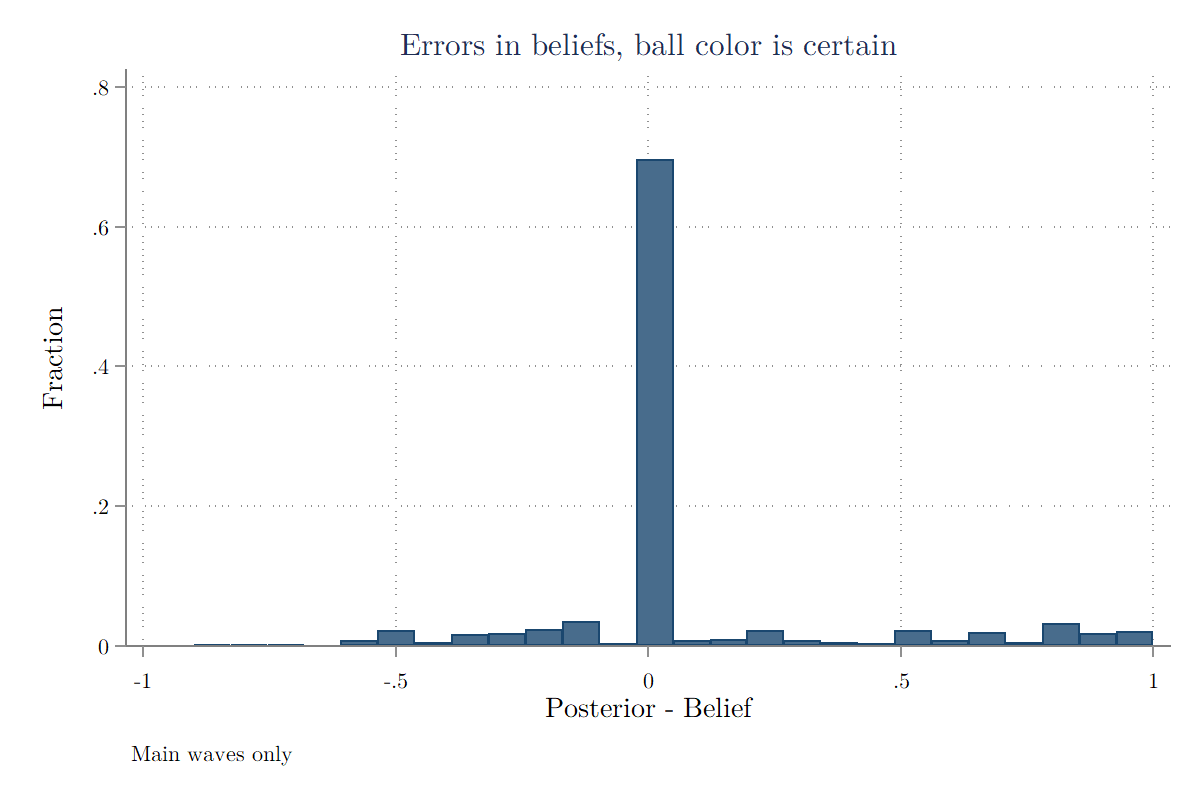
\includegraphics[width=.48\textwidth]{Graphs/hist_belief_error_s5.png}}
	\hfill
	\subcaptionbox{Error v. Posterior, Certain Posterior}{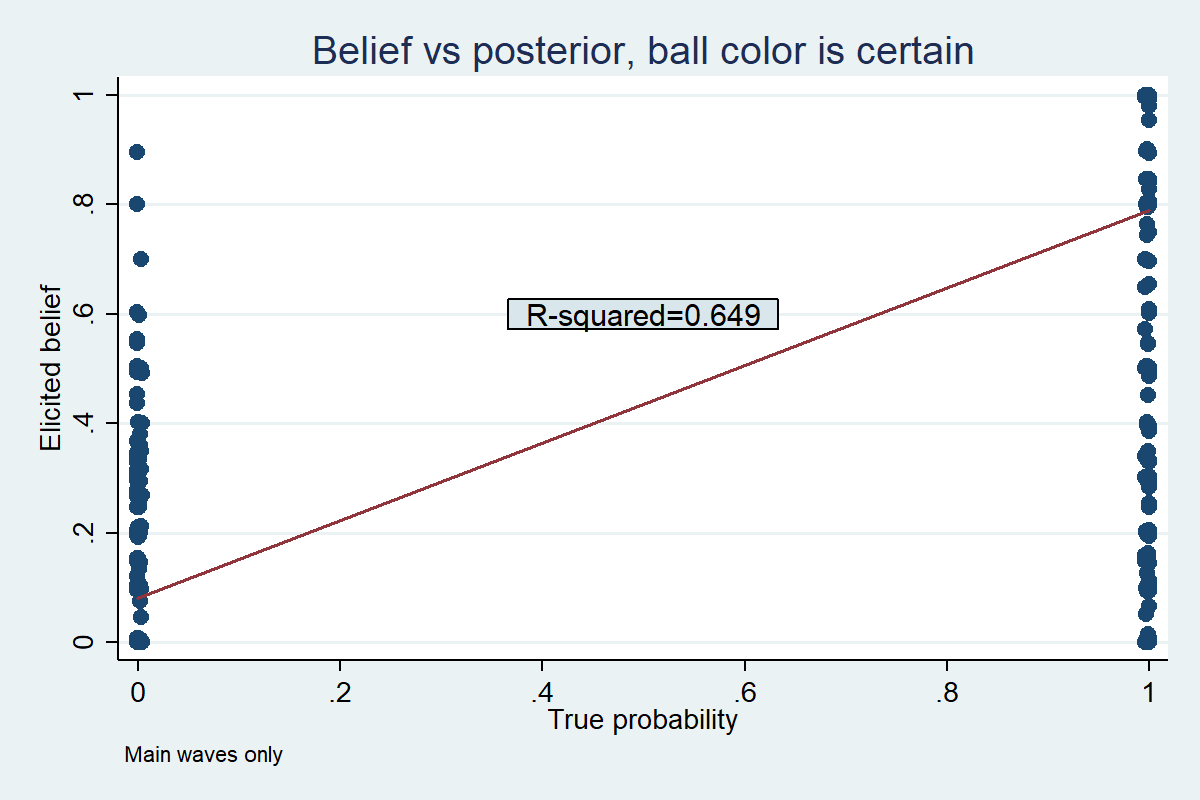
\includegraphics[width=.48\textwidth]{Graphs/updating_s5.png}}
	\hfill
	\vspace{2em}
	\subcaptionbox{Error Distribution, Uncertain Posterior}{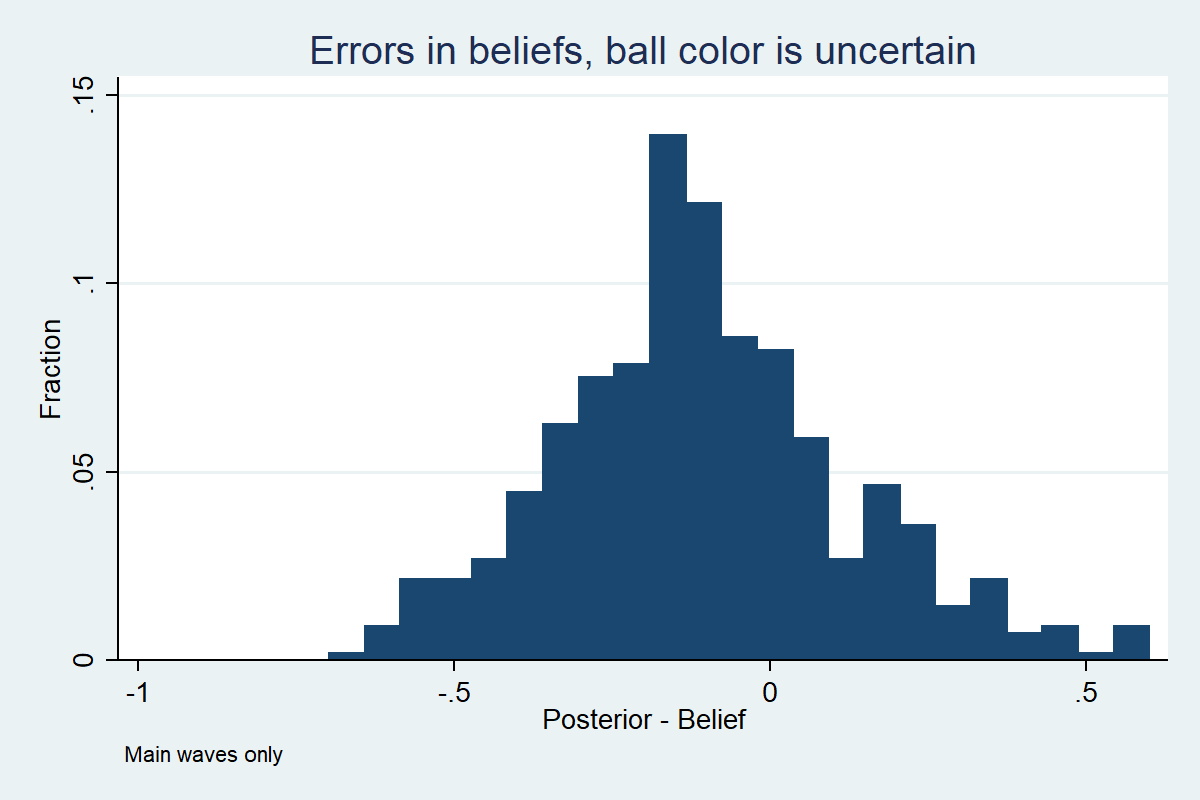
\includegraphics[width=.48\textwidth]{Graphs/hist_belief_error_s4.png}}
	\hfill
	\subcaptionbox{Error v. Posterior, Uncertain Posterior}{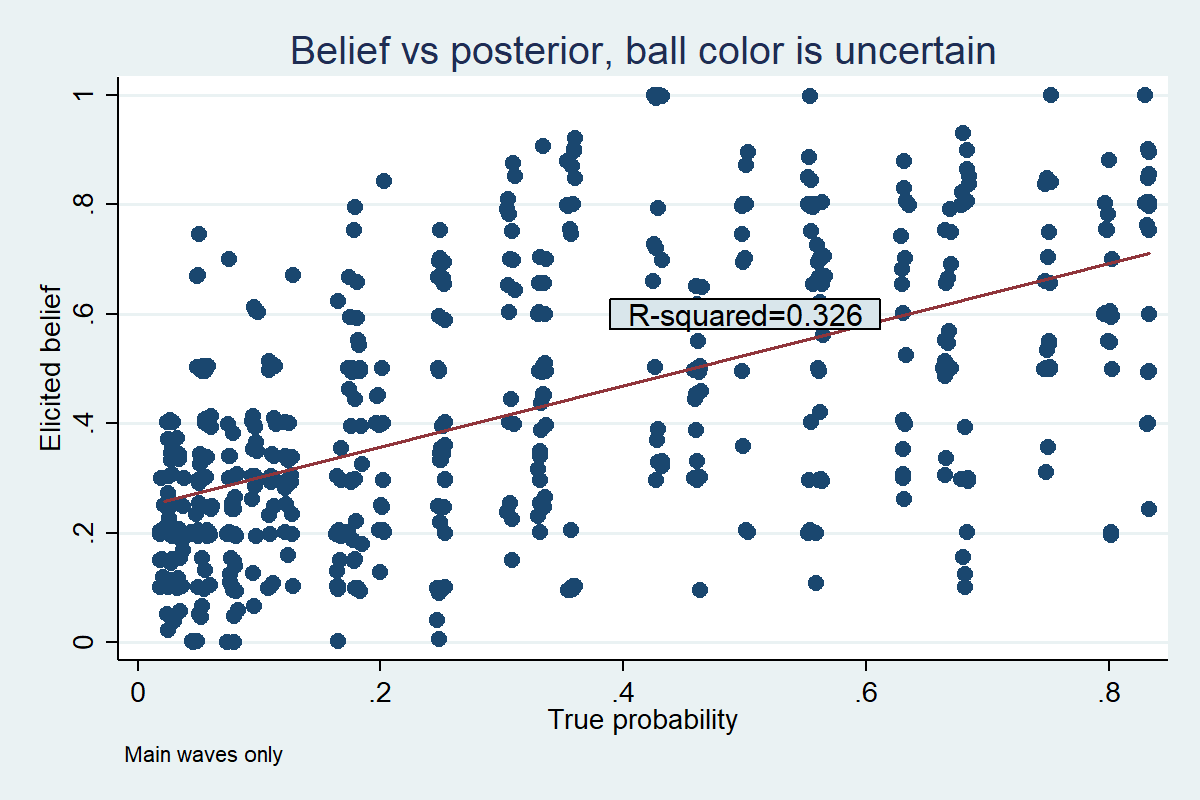
\includegraphics[width=.48\textwidth]{Graphs/updating_s4.png}}
	\hfill
\end{figure}
%%%%%%%%%%%%%%%%%%%%%%%%%%%%%%%%%%%%%%%%%%%%%%%%%%%%%%%%%%%%%%%%%%%%%%%%%%%%%%%%%%%%%%%%%%%%%%%%%%%%%%%%%%%%%%%%%%%

We define updating errors as the difference between the posterior and subjects' elicited belief of the posterior probability of drawing a black ball for a given signal.  The left-hand column of Figure~\ref{fig:BeliefUpdate} shows the distribution of the updating errors, while its right-hand column presents a scatter plot of the elicited beliefs against the true posterior with a fitted line.
%Since subjects were only given signal characteristics and not true posteriors, their IP responses reflect, inter alia, their ability to infer the true posteriors from signal characteristics. (I'm not sure I like my sentence better)
Panel A uses all observations and suggests that, while errors occur, beliefs are still sensible. The distribution of updating errors is centered at 0, with roughly one-half (51\%) concentrated within +/- 0.1 interval around zero. Overall, the correlation between the elicited beliefs and the true posteriors was 0.653.  

Some combinations of priors and signals correspond to completely certain posteriors where updating should be trivial.  
%Panel B includes only the 44\% beliefs elicited for an uncertain posterior. 
Panel~B plots such cases, which account for 56\% of the sample and includes: (i) treatments with all-honest gremlins; and (ii) treatments with obviously irrelevant dishonest gremlins (e.g., a gremlin from a group with honest and white-swamp gremlins announcing that the ball is black --- or vice versa). Reassuringly, 69\% of reported beliefs are correct. About half of the errors involve reporting a probability of one when it should have been zero.

Meanwhile, Panel~C plots difference excluding observations with certain posteriors. The median error in Panel C is -0.12, with with 90\% of errors lying between -0.48 and 0.3, suggesting that, on average, subjects overestimate the likelihood of adverse events for uncertain posteriors. The correlation between beliefs and posteriors in this sub-sample falls to 0.571.\footnote{The overall pattern of belief updating is consistent with the existing literature which shows that despite updating in the correct direction, people tend to underreact both to the priors and to the signals. The effect of underweighting priors --- first noted in the psychology literature \citep*{phillips_conservatism_1966-1, tversky_belief_1971, kahneman_subjective_1972} --- is known as \emph{representativeness bias} or \emph{base-rate neglect}. Using the regression approach of \citet{grether_bayes_1980}, we find both base-rate neglect and signal underweighting. Our estimates of these parameters are significantly below one with $\hat \alpha=0.43$ $\hat \beta=0.25$ (see Column 1 in \ref{belief_decomposition}). These values are within the range found by the meta-analysis of \citet{benjamin_chapter_2019} which calculates the average $\hat \alpha$ estimate to be around 0.22 (0.4 for incentivized studies only) and the average $\hat \beta$ to be 0.6 (0.43 for incentivized) for studies (like ours) that presented their signals simultaneously.  The common name for this kinds of experiments is \emph{bookbag-and-poker-chip experiments}} 

%%%%%%%%%%%%%%%%%%%%%%%%%%%%%%%%%%%%%%%%%%%%%%%%%%%%%%%%%%%%%%%%%%%%%%%%%%%%%%%%%%%%%%%%%%%%%

\begin{table}[H]\centering 
\caption{Average Updating Error by Signal Type} 
\label{tab:nonparError}
\adjustbox{max width=\textwidth}{
	\begin{threeparttable}
	\begin{tabular}{ccccccc} 
	\hline \hline
 \multirow{4}{6ex}{\centering \textbf{Row}}& \multicolumn{3}{c}{\centering \textbf{Signal Characteristics}}
			& \multirow{3}{10ex}{\centering \textbf{Posterior}}  
			& \multirow{3}{12ex}{\centering \textbf{Updating Error$^*$}} & \multirow{3}{12ex}{\centering \textbf{P-val $(H_0: Error = 0)$}}  \\ \cmidrule(lr){2-4}
		& \multirow{2}{10ex}{\centering \textbf{False Positive}} & \multirow{2}{12ex}{\centering \textbf{False Negative}} 
			& \multirow{2}{10ex}{\centering \textbf{Signal}} 
		\\
		\\
		& (1) & (2) & (3) & (4) & (5) \\
	
		\hline	
(1)&No&No&White&0.000&0.050&0.000\\
(3)&No&Yes&White&0.100&0.122&0.000\\
(5)&Yes&No&White&0.000&0.122&0.000\\
(7)&Yes&Yes&White&0.131&0.218&0.000\\
(2)&No&No&Black&1.000&-0.163&0.000\\
(4)&No&Yes&Black&1.000&-0.279&0.000\\
(6)&Yes&No&Black&0.550&0.039&0.130\\
(8)&Yes&Yes&Black&0.483&0.048&0.021\\

\\ 	[-1em]
\hline\hline
\end{tabular} 
	\begin{tablenotes}[flushleft]
			\item\leavevmode\kern-\scriptspace\kern-\labelsep \footnotesize \textit{Notes:} $^* \text{Updating error} = Posterior - Belief$. 
	\end{tablenotes}								
	\end{threeparttable}
	}
\end{table}
%%%%%%%%%%%%%%%%%%%%%%%%%%%%%%%%%%%%%%%%%%%%%%%%%%%%%%%%%%%%%%%%%%%%%%%%%%%%%%%%%%%%%%%%%%%%%



Table~\ref{tab:nonparError} summarizes how updating errors vary with signal characteristics. We find that subjects overestimate the probability of a black ball when they received a white signal, and introducing FP rates to the signal exacerbates this upward bias. To illustrate, consider the change between rows 1 and 3, where introducing a FP rate would not change the posterior because the signal is white. Yet, subjects update their posterior upward, magnifying their updating error. FN rates have a similar effect of exacerbating this upward bias for a white signal.

The updating bias for black signals, however, varies by the information structure. Subjects slightly underestimate the probability even when the signal is honest, but introducing FN rates leads subjects to underestimate it further. To illustrate, the introduction of a FN rate given a black signal does not change the posterior (rows 5 and 6), but subjects' beliefs decrease. When there is a risk of a false-positive (i.e., FP$>$0), subjects again overestimate the probability of a black ball with little difference in errors between treatments with FP events only and with both FP and FN events. It seems that as the false-positive rate negatively affects the posterior, subjects fail to adjust their beliefs enough in response to FP rates.


\vspace{20pt}

\section{WTP and Signal Characteristics}\label{sec:results}

\subsection{Are Subjects Risk Neutral, Expected Utility Maximizers?} 

\begin{hypothesis}\label{hyp:eqRN} 
Subjects' WTPs for signals are equal to their value for risk-neutral agents. 
\end{hypothesis}

\begin{result} 
On average, there are no significant discrepancies between WTP and predicted value for risk-neutral agents. When splitting by a signal type, the difference emerges only for signals with both false-positive and false-negative events.
\end{result}

\begin{hypothesis}\label{hyp:eqSen} 
Subjects' preferences demonstrate equal sensitivity to costs generated by false-positive and false-negative events. 
\end{hypothesis}

\begin{result} 
On average for our signal and sample structure, we cannot reject the hypothesis of equal sensitivity. However, we observe significant heterogeneity with respect to priors: subjects tend to overvalue false-negative costs for low probability events and overvalue false-positive costs for high probability events. 
\end{result}





%The model provides a simple benchmark to evaluate potential welfare gains from the signal. Depending on the assumptions on signal characteristics and risk preferences, agents can pay more or less than the risk-neutral benchmark.
%
%We next examine whether subjects understand the WTPE task. One of the model's basic prediction is that signal value decreases with false positive and false negative rates. If subjects understand the basic premise of the WTPE, then we expect a negative correlation between the WTP and the signal's false positive and false negative rate. 

Overall, the theoretical value of a signal for a utility maximizing risk-neutral subject (hereafter, risk-neutral signal value) in equation~\ref{eq:rnWTP} appears to be a useful benchmark of our subjects' WTP. Figure~\ref{fig:WTPhist} plots the distribution of the differences between subjects' WTP and the signal value.  
%WTP is bounded between \$0 and \$5, where the latter is because protection can be purchased for \$5 so if information were that valuable, an individual would just choose to protect.  
The WTP is centered around the risk-neutral signal value, indicating that average choices do not fall far from the choices of a risk-neutral utility maximizer. However, there is substantial variation: only 25\% of reported WTP are within \$0.50 of the risk-neutral signal value, and subjects overvalue signals by at least \$1.5 in 22\% of cases and undervalue by at least \$1.5 in 19\% of cases. Introducing FP and FN rates doesn't increase the range or variation of discrepancies, but introduces a long tail of positive discrepancies shifting the average up.


\begin{figure}[H]\centering 
	\caption{Discrepancy (Observed WTP - Signal value) by Signal Type} \label{fig:WTPhist}
	\subcaptionbox{All signals}{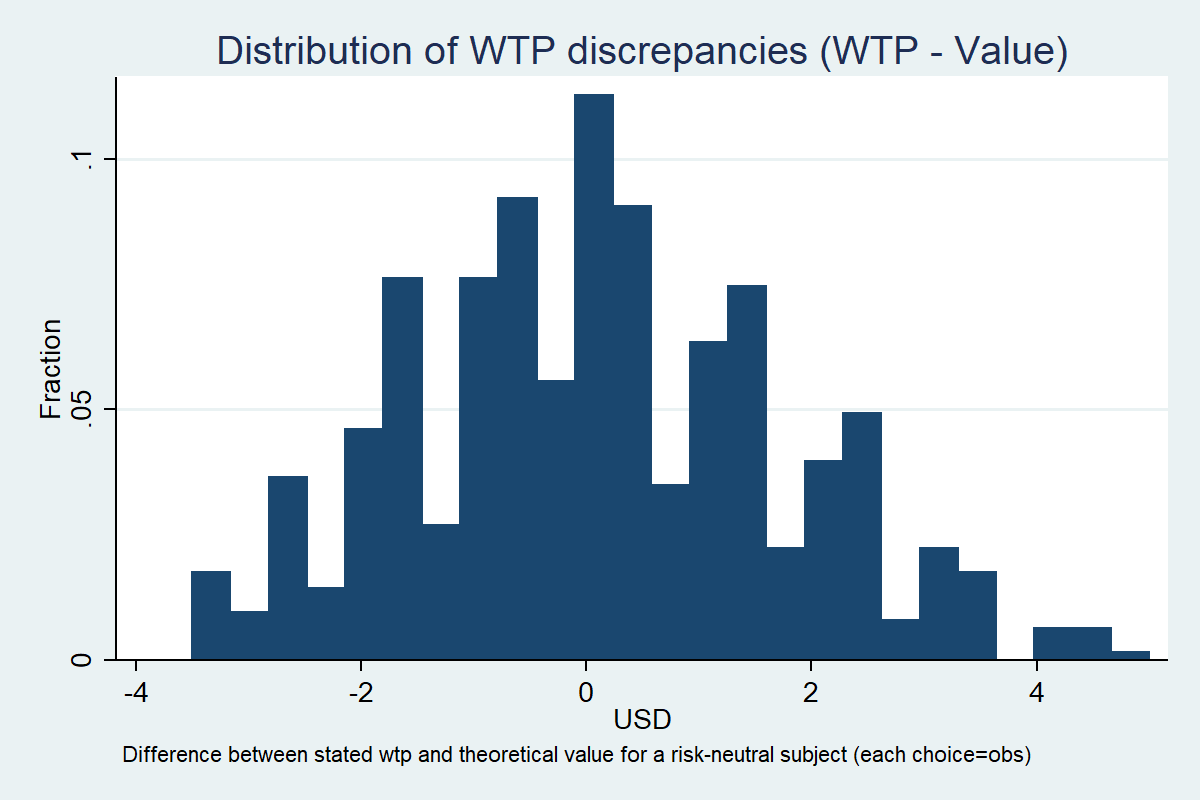
\includegraphics[width=.48\textwidth]{Graphs/hist_WTP_discr1.png}}
	\hfill
	\subcaptionbox{FP only}{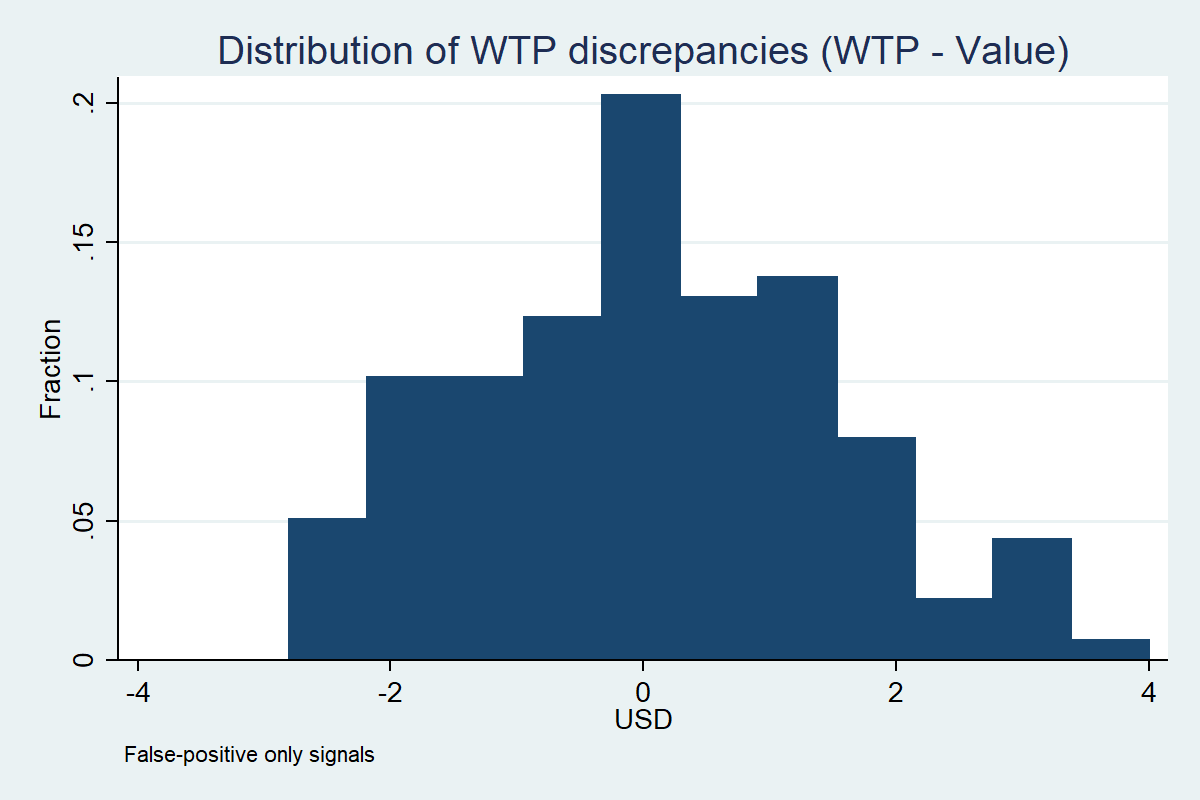
\includegraphics[width=.48\textwidth]{Graphs/hist_WTP_discr1fp.png}}
	\hfill
	\vspace{2em}
	\subcaptionbox{FN only}{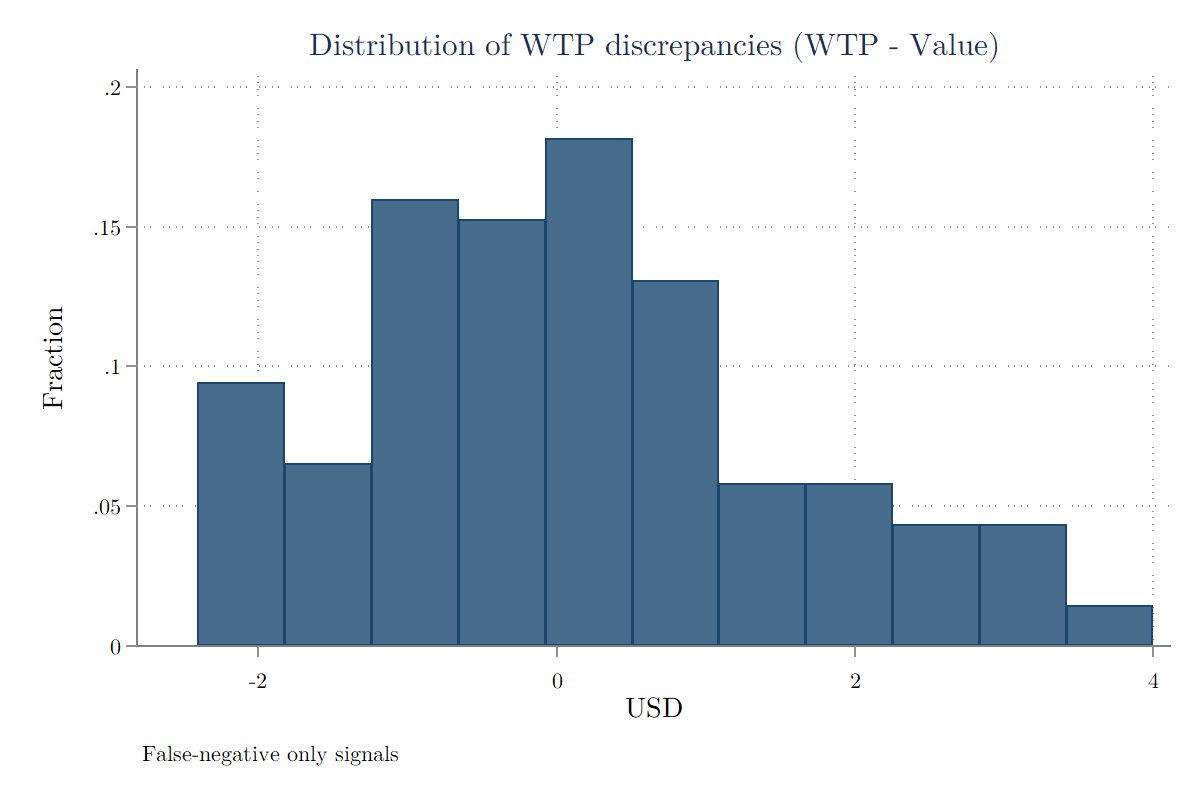
\includegraphics[width=.48\textwidth]{Graphs/hist_WTP_discr1fn.png}}
	\hfill
	\subcaptionbox{Both FP and FN}{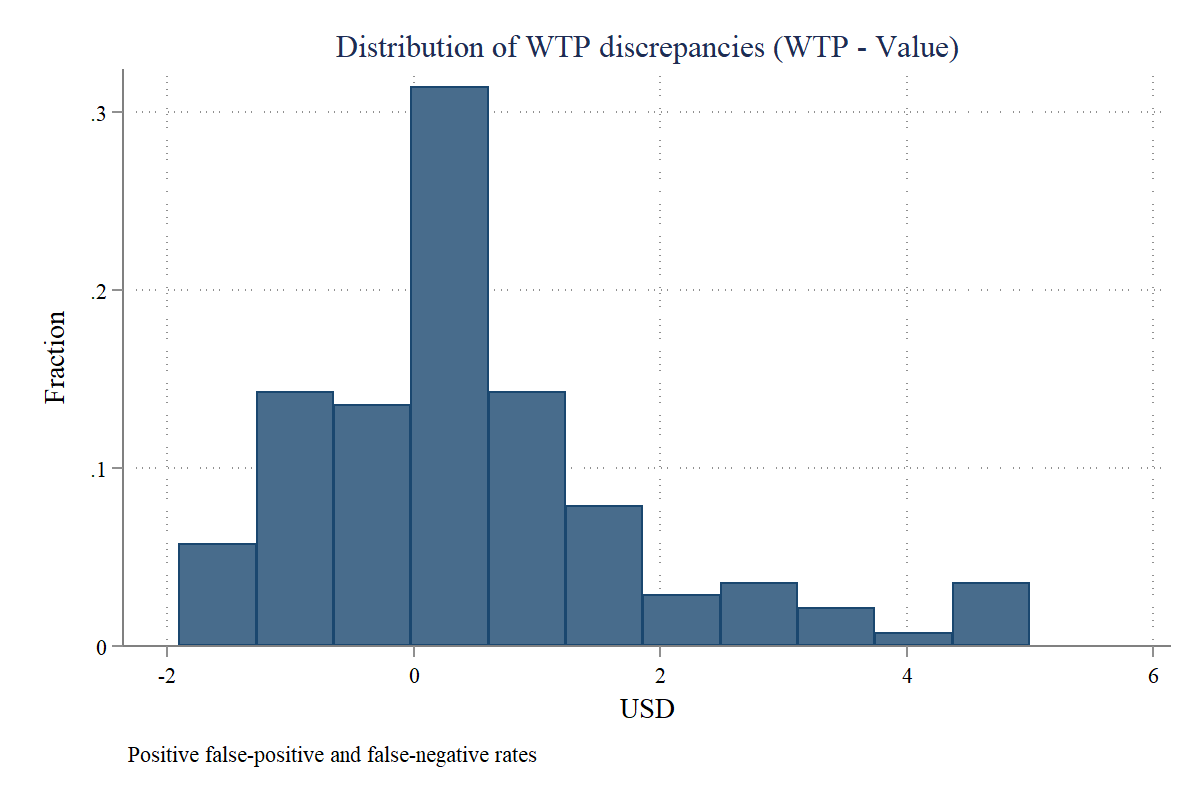
\includegraphics[width=.48\textwidth]{Graphs/hist_WTP_discr1fpfn.png}}
	\hfill

\end{figure}

Our non-parametric analysis in Table~\ref{tab:WTP_nonpar} also finds no differences on average between the observed WTP and the risk-neutral signal value for 3 out of 4 broad categories of signal characteristics: honest signals; signals with only false-positive events; and signals with only false-negative events. When there are both false positives and false negatives, however, subjects significantly overvalue signals relative to the theoretical benchmark. We observe overvaluing both for low and high priors with roughly the same average difference and at the same statistical significance level. Note, that these signals also tend to cause overprotection in the IP task. Subjects also tend to overpay for signals with positive FP rates when the prior is low, and for the signals with positive FN rates when the prior is high (0.3 or 0.5).


%%%%%%%%%%%%%%%%%%%%%%%%%%%%%%%%%%%%%%%%%%%%%%%%%%%%%%%%%%%%%%%%%%%%%%%%%%%%%%%%%%%%%%%%%%%%%%%%%

%\begin{table}[H]\centering \caption{Average WTP discrepancy (WTP-Value) by Signal Type} \label{WTP_nonpar} \begin{tabular}{cccc} \hline \hline
\multirow{2}{12ex}{\centering \textbf{False positive}}&\multirow{2}{12ex}{\centering \textbf{False negative}}&\multirow{2}{15ex}{\textbf{\centering Mean WTP discrepancy}}& \multirow{2}{10ex}{\centering \textbf{P($=0$)}}\\ 
\\
\hline
No&No&-0.106&0.433\\
No&Yes&0.143&0.250\\
Yes&No&0.081&0.502\\
Yes&Yes&0.492&0.000\\
\hline \end{tabular} \end{table}


\begin{table}[H]\centering \caption{Average WTP discrepancy (WTP-Value) by Signal Type} \begin{tabular}{ccccc} \hline \hline
\textbf{Priors}&\textbf{Honest}&\textbf{FN only}& \textbf{FP only} & \textbf{FP and FN}\\ \hline
All priors&-0.106&0.143&0.081&0.492***\\
Low priors&-0.135&-0.209&0.465**&0.437**\\
High priors ($>$0.2)&-0.077&0.496*&-0.303&0.547**\\
\hline \\ \end{tabular} \end{table}


%To understand how subjects' WTP deviates from these risk-neutral signal value, we use a regression analysis of discrepancies between reported WTP and theoretical values to understand, first, the validity of a risk-neutral model and, second, relative weights put on false-negative and false-positive costs. 

We estimate the relationship between WTP biases and signal characteristics more formally with the following regression:
\[\Delta b_{is} = \beta_0 + \beta_1 FP + \beta_2 FN + \varepsilon_{is}\]
where $\Delta b_{is} = (b_{is} - b^*_s)$ is the difference between the WTP of individual $i$ for signal $s$ and $b^*_s$ is the signal value; FP (FN) is the false positive (false negative) cost. All specifications include subject fixed effects, with standard errors clustered at the subject level. If subjects are risk-neutral expected-utility-maximizers, we expect $\beta_1=0$ and $\beta_2=0$. The result, reported in column 1 of Table~\ref{tab:wtp_ols}, shows positive and statistically significant coefficients for both FP and FN costs. In other words, subjects deviate from the benchmark model and overpay for inaccurate signals. 


%\subsection{The (As-)symetry of False Positive and False Negative Signals} 

%First, subjects' WTPs for a signal are equal to its value for risk-neutral agents. The model provides a simple benchmark to evaluate potential welfare gains from the signal. Depending on the assumptions on signal characteristics and risk preferences, agents can pay more or less than the risk-neutral benchmark.
%
%Second, subjects' preferences value the marginal costs from false-negative and false-positive information equally. The model of a risk-neutral agent suggests that they should. Our derivations above indicate that the relative weight of false-negative costs can be either below or above one depending on risk preferences only.

%\begin{hypothesis}\label{hyp:eqRN} 
%Subjects' WTPs for a signal are equal to its value for risk-neutral agents. 
%\end{hypothesis}

%%%%%%%%%%%%%%%%%%%%%%%%%%%%%%%%%%%%%%%%%%%%%%%%%%%%%%%%%%%%%%%%%%%%%%%%%%%%%%%%%%%%%%%%%%%%%%%%%

\begin{table}[htbp!]
\centering
\adjustbox{max width = \textwidth}{
	\begin{threeparttable}
	\caption{Deviations from Signal Value (WTP - Value) and Signal Characteristics}
	\label{tab:wtp_ols}
	\begin{tabular}{l*{5}{c}}
		\hline\hline
		&\multicolumn{3}{c}{\multirow{2}{*}{All}} & \multicolumn{2}{c}{Prior}\\ \cmidrule(lr){5-6}
		&&&& $\{.1,.2\}$ & $\{.3,.5\}$\\ 
		\cmidrule(lr){2-4} \cmidrule(lr){5-5} \cmidrule(lr){6-6}  
		&\multirow{1}{*}{(1)} & \multirow{1}{*}{(2)} & \multirow{1}{*}{(3)} & \multirow{1}{*}{(4)} & \multirow{1}{*}{(5)}\\
	\hline
	\\ [-0.5em]
		\exInput{Tables/wtpdiff_ols.tex}
				\hline
		Subject FE & Yes & Yes & Yes & Yes & Yes \\
		Inaccurate Belief Interactions & No & No & Yes & Yes & Yes \\
		Prior Probability FE & No & No & No & Yes & Yes \\
		\hline\hline
	\end{tabular}
	\begin{tablenotes}[flushleft]
		\item\leavevmode\kern-\scriptspace\kern-\labelsep \small\textit{Notes:} Standard errors in parentheses. \sym{*} \(p<0.10\), \sym{**} \(p<0.05\), \sym{***} \(p<0.01\).
	\end{tablenotes}
	\end{threeparttable}
}
\end{table}		

		
%%%%%%%%%%%%%%%%%%%%%%%%%%%%%%%%%%%%%%%%%%%%%%%%%%%%%%%%%%%%%%%%%%%%%%%%%%%%%%%%%%%%%%%%%%%%%%%%%


The risk-neutral model also predicts that subjects should value the marginal costs of false-negative and false-positive events symmetrically. \aut{We find (Table~\ref{tab:wtp_ols}) that the coefficient on FN costs is slightly larger indicating higher sensitivity to FP costs, but we cannot reject the hypothesis that the two coefficients are equal. However later we note that this equivalency breaks down when considering specific priors.}

\subsection{Risk Preference and Belief Accuracy}

Our baseline estimation in column 1 indicates significant deviations from the model's predictions. Positive and significant coefficients on FP and FN costs indicate that subjects reduce their WTP with growing FP and FN rates by less than a risk-neutral decision-maker would, i.e., subjects tend to overvalue signals of poor quality.

As our benchmark model assumes both perfect updating and risk neutrality, assumptions which open two channels through which deviations could occur. First, Proposition~\ref{thm:riskAverse} suggests that risk preferences can influence the sensitivity of WTP to these signal characteristics. Second, systematic biases during the updating process can also lead to deviations. 

We find that risk preferences matter for sensitivity to signal characteristics. We use data from the BP task to categorize subjects by their risk preference. We classify all the subjects with internally consistent BP choices into three risk-preference categories: risk averse, risk neutral, and risk loving.\footnote{We classify subjects based on the total number of protection choices made in the BP task with 2 or 3 choices corresponding to risk-neutrality (protecting starting from 0.2 or 0.25), but exclude subjects making more than one choice at odds with a consistent risk preference.} Column 2 explores the heterogeneity of subject responses to FP and FN costs by their risk preferences, with risk-neutral as the default category. The point estimates for risk-neutral subjects are actually a bit larger than those of the average subjects (column 1) and indicate higher bias. Risk-averse subjects have lower extra sensitivity to FP and FN costs indicating lower bias. In fact, their total sensitivity to FP and FN costs is almost exactly zero. Risk-loving subjects do not significantly differ from the risk-neutral ones. 

Accounting both for belief accuracy and for risk preferences also does little to explain the pattern of underreacting to FP and FN rates. To study the role of subjects' ability to Bayesian update, we use data from the BE task to categorize the WTP responses by belief accuracy.\footnote{We calculate a belief error as the absolute value of the difference between the subject's belief and the true posterior probability and then average these errors across all the decisions with identical priors, false positive and false negative rates. A subject's posterior belief for a decision is defined as accurate if its error is less than the median error across all the subjects making the same decision.} Column 3 presents the most flexible specification that controls for belief accuracy and risk preference by including triple interactions of belief accuracy, risk preference, and signal characteristics. The baseline group is the group of risk-neutral subjects with relatively accurate beliefs. We find a lower sensitivity to FP costs for risk-neutral subjects with accurate beliefs and very little change to the corresponding sensitivity to FN costs. This indicates that even subjects with accurate beliefs still underreact to changing FP/FN costs.\footnote{Aside from these theoretically motivated individual differences, we investigate several other characteristics.  Heterogeneity is not driven by demographic characteristics (e.g., age, gender) or prior statistical coursework.  These results are in Appendix A Table~\ref{wtp_dem}.}
  

\subsection{Heterogeneity by Prior}

We motivate our experiment with real world problems of designing signals for low-probability disasters. With a low prior, the default action of risk-neutral subject would be not to protect, and vice versa with a high prior. The signal would help risk-neutral subjects decide whether to keep the default action or to switch. We split the prior by below/above 0.25 (= protection cost/potential loss).  We incorporate prior-probability fixed effects to the aforementioned flexible specification. 

Column 4 presents the results for low-prior WTPE tasks. With a low prior, subjects undervalue false positive costs relative to the risk-neutral baseline. In other words, with low priors, subjects overvalue signals that would induce them to overprotect. This overvaluation is similar for different risk preference profiles. Both risk-averse and risk-loving subjects tend to underreact to FP costs, while risk-averse tend to overreact to false-negative latter which is consistent with our theory. It should be noted that while coefficients' magnitudes are relatively large, none of the coefficients or predicted sensitivities here (bottom panel) is significant due to relatively small sample size, so these results should be interpreted very cautiously. 

Column 5 presents the results for high-prior WTPE tasks. With a high prior, both risk-neutral and risk-loving subjects become less sensitive to FN costs and reduce their WTP less per dollar of expected false-negative costs as indicated by positive and significant coefficient. These results imply a slight tendency to overvalue signals that would induce them to underprotect. At the same time, the coefficient on FP costs goes down indicating higher sensitivity to FP costs. Risk-averse subjects even overreact to false-positive cost though the effect is not significant given our sample size. 

To sum up, most subjects underreact to false-positive costs with low priors, but underreact to false-negative rates for high priors. In practice, and given low priors implied by many alert systems, it means that users would tend to overpay for alert signals with high false-positive costs, while excessively discounting signals with significant false-negative rates. For example, they would prefer a smoke alarm which never misses fires even if it involves higher expected costs of false alarms. Risk preferences seem to affect this pattern with risk-averse subjects moving closer to a risk-neutral benchmark, but most interaction coefficients are not statistically significant despite high magnitudes.

%While this finding is incidental and not the part of the original research plan, its significant practical implications prompt us to explore it further.



%XXX \agt{ALL: What would be nice if we can derive how higher prior would affect risk-averse/loving subjects. Also let's discuss what this really means and how to interpret. Does this mean that people overvalue signals that would change their default action?} \aut{It would be nice, but it does not seem currently possible in general case except the results already given in the theory section.} XXX


%There is also a possibility that the sensitivity is affected by subjects' demographic characteristics or their statistical education. 
%We find little evidence for heterogeneous effects by demographic characteristics or statistical education. We show in (Appendix A  Table~\ref{wtp_dem}) that gender or previous statistical education do not have significant effects on sensitivities for false-positive and false-negative rates. We find weak evidence that older (23+) subjects have a lower WTP for signals though the age variation is pretty limited. 
%Generally, the heterogeneity analysis is potentially constrained by  



%\subsection{Discussion: What Accounts for the Heterogeneity by Prior?}
\section{Heterogeneity by Prior}

Many real-life examples of alerts such as fire alarms and mammograms have low priors. Hence it is important to explain the pattern of under-reaction to false-positive rates for low priors to see if this explanation extends to real life and if the explanation indicates any tools to manipulate this response.

Before going to explanations, we need to make sure, first, that the pattern is robust and, second, that it holds for the original WTP data and not only for the differences with the benchmark value. We estimate directly the regression of reported willingness-to-pay on false-positive and false-negative rates given to subjects directly (Figure ~\ref{fig:Comparison}). We find that the sensitivities to both false-positive and false-negative rates increase with priors and that the change occurs relatively smoothly. Two sensitivities are also surprisingly close to each other.\footnote{For none of the priors can we reject the hypothesis that two sensitivities are equal to each other.} This drastically contrasts with the risk-neutral model, predicting that the sensitivity to FP rates should be much higher than the sensitivity to FN rates for low priors, but lower for high priors. This happens because for a given FN rate, false-negative events are much less likely with low priors and hence impose less costs on the agent. Increasing priors in theory makes FN rates more salient while the saliency of FP rates should go down. This discrepancy between WTP and the theoretical value explains changing signs on FP and FN costs in the previous regressions of WTP differences. Hence the puzzle can be reframed as the uniformity of WTP response to FP and FN rates for different priors.

%\begin{table}[htbp]\centering
\def\sym#1{\ifmmode^{#1}\else\(^{#1}\)\fi}
\caption{WTP for Information, by prior (tobit)}
\begin{tabular}{l*{4}{c}}
\hline\hline
                &\multicolumn{1}{c}{(1)}&\multicolumn{1}{c}{(2)}&\multicolumn{1}{c}{(3)}&\multicolumn{1}{c}{(4)}\\
                &\multicolumn{1}{c}{0.1}&\multicolumn{1}{c}{0.2}&\multicolumn{1}{c}{0.3}&\multicolumn{1}{c}{0.5}\\
\hline
model           &                  &                  &                  &                  \\
FP rate         &    -2.91\sym{***}&    -2.08\sym{**} &    -4.46\sym{***}&    -3.25\sym{**} \\
                &    (1.1)         &    (1.0)         &    (1.0)         &    (1.3)         \\
FN rate         &    -2.48\sym{**} &    -2.73\sym{***}&     -3.7\sym{***}&    -3.65\sym{***}\\
                &    (1.1)         &    (1.0)         &    (1.0)         &    (1.3)         \\
Constant        &     1.79\sym{***}&     2.33\sym{***}&     2.71\sym{***}&     3.32\sym{***}\\
                &    (0.2)         &    (0.2)         &    (0.2)         &    (0.3)         \\
\hline
sigma           &                  &                  &                  &                  \\
Constant        &     1.83\sym{***}&      1.7\sym{***}&     1.72\sym{***}&     2.16\sym{***}\\
                &    (0.1)         &    (0.1)         &    (0.1)         &    (0.2)         \\
\hline
P(FP rate=FN rate)&     .792         &     .669         &     .617         &     .832         \\
Adjusted \(R^{2}\)&        .         &        .         &        .         &        .         \\
Observations    &      159         &      153         &      159         &      153         \\
\hline\hline
\multicolumn{5}{l}{\footnotesize Standard errors in parentheses}\\
\multicolumn{5}{l}{\footnotesize \sym{*} \(p<0.10\), \sym{**} \(p<0.05\), \sym{***} \(p<0.01\)}\\
\end{tabular}
\end{table}
\label{tobit_het}

\begin{figure}[H]
\centering
\caption{Theoretical and Empirical WTP Sensitivities to FP and FN rates} \label{fig:Comparison}
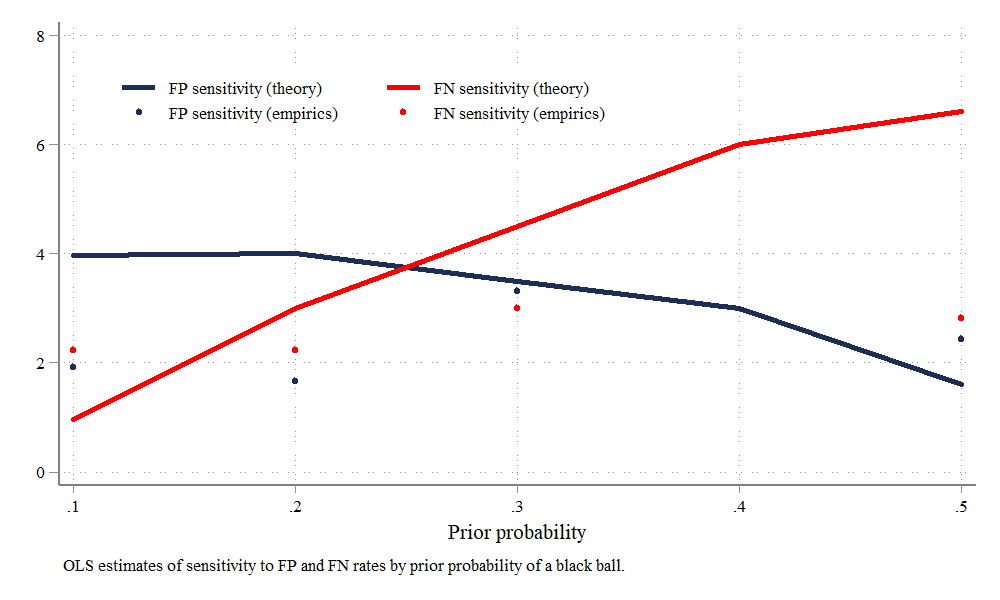
\includegraphics[width=0.8\textwidth]{Graphs/sensit_comparison.png}
\end{figure}




There are several candidate explanations for the observed pattern. Fist, we know that risk preferences affect sensitivities to FP and FN rates making them a natural candidate. Second, the heterogeneity could be caused by subjects putting some value on non-instrumental information or signals that do not change their actions. Third, the pattern can emerge due to some subjects failing to account for changes in prior probabilities between rounds (anchoring).  Finally, the choices we observe are consistent with subjects neglecting the difference between false-positive and false-negative signals (black-eyed and white-eyed gremlins in the presentation) leading to similar coefficients on FP and FN rates and less changes of coefficients with priors. 

%We start with the most a priori probable explanation of risk preferences. 
Proposition 3 predicts that risk averse subjects have a stronger reaction to false-negative costs as compared to risk-neutral subjects, but our sample includes both risk-averse, risk-neutral, and risk-loving individuals, hence the average response need not follow any of the patterns consistent with uniform risk-aversion. We test the risk preferences explanation using subjects' BP choices. If subjects express the same risk preferences across tasks, then accounting for these choices should either explain away the observed heterogeneity pattern or significantly reduce it. It is already obvious from Columns (4)-(5) in Table~\ref{tab:wtp_ols}, where coefficients on FP and FN costs are very different for low and high priors. We augment this analysis in Table~\ref{wtp_het_risk} by explicitly testing for interactions between risk-preferences, priors, and false-positive and false-negative rates. We find that these interactions are mostly insignificant, with the exception of interactions between false-negative rates and risk aversion for some specifications. The heterogeneity largely remains after controlling for risk preferences, but the interaction between high priors and false-positive rates becomes insignificant.

The evidence does not support subjects anchoring on previous priors or from preferences for non-instrumental information. Each subject goes through two sets of treatments with two different priors and a fixed order of priors, so anchoring could be possible.  We find, however, that most subjects (92 out of 104) change their decisions when going from one prior to another, and the average belief error in the BE task is actually \itshape{lower}\normalfont for the second set of priors rather than the first, which suggests that changing priors does not increase subjects' confusion. Most importantly, the uniformity in coefficient ratio is present even if we limit our attention only to the first priors in each sequence.\footnote{Depending on session, the first 3 WTP treatments use either 0.1 or 0.2 as the prior, so there is no anchoring on the previous prior or something special about a particular prior.}

\aut{There is certainly evidence that people value information that does not affect their decisions \citet{eliaz_paying_2010, masatlioglu_intrinsic_2017}, i.e., non-instrumental information. Most information in our experiment is instrumental by design (it helps to choose actions) and indeed enters into subjects' decisions as evidenced by choices in the IP task. However, we also observe many subjects choosing positive WTP for signals not affecting their IP decisions (159 out of 624 total choices), so it is plausible that the reported WTP includes some non-instrumental component. We still believe that preferences for instrumental information cannot provide a full explanation of our results.  First, the sensitivity of WTP to FP rates is much lower in the experiment compared to the theory when priors are low. Suppose that the value of information is given by $b(\pi,P_{01},P_{10})+n(\pi,P_{01},P_{10})$ with $n()$ describing the non-instrumental component. If this discrepancy in sensitivities to FP rates comes from the non-instrumental component $n$, it needs to be increasing in FP rates. In other words, subjects should put higher non-instrumental value on worse signals which seems implausible. Second, the closeness of coefficients for FP and FN rates seems also apriori implausible based only on the non-instrumental information value story.}

For our preferred explanation, we use subjects' own proffered explanation.  At the end of the experiment, we asked subjects to explain to us how they made their protection choices.  Out of 105 subjects in the main waves of the experiment, 39 refer to the \textit{percentage} \normalfont  of dishonest gremlins as their rationale for choosing protection.\footnote{IS IT POSSIBLE TO PUT A TABLE IN THE APPENDIX WITH THESE STATEMENTS, WITH THOSE IN YOUR 39 HIGHLIGHTED?}  For example,\\
\textit{"I took into consideration how many honest there were and looked at the chances of picking a ball."}\\
\textit{"If there were only honest gremlins then I never protected but even if there was one white-swamp gremlin or one black-swamp gremlin then I payed for protection."}\\
Among the other 66 subjects, some may use this heuristic without describing it.  The closeness of the coefficient estimates for FP and FN rates in Table ~\ref{tobit_het} are certainly consistent with these statements. If subjects neglect the difference between false-positive and false-negative risks when choosing their WTP, it would explain both the coefficients' similarity and their lack of variation with respect to priors. Indeed, if subjects treat FP and FN rates the same and consider only the total proportion of false signals, they would assign equal weights to each of them, and the best fit line of signal's value with the respect to the sum of FP and FN rates should be relatively flat because priors affect FP and FN costs in opposite ways. Note also that the equality of coefficients on FP and FN rates is a necessary prediction of this explanation, but can emerge only by chance with (some) heterogeneous risk preferences.

In order to test this hypothesis, we use choices from the BE and IP tasks where subjects also face imperfect signals. If subjects systematically neglect the difference between FP and FN rates, we expect to find the pattern of unexplained reaction to FP and FN rates in cases when they do not affect the posterior. Namely, subjects would show sensitivity to FP rates when the signal is white and sensitivity to FN rates with black (positive) signals. This happens because some subjects react to FP rates as if they are FN rates, and vice-versa. If present, this pattern cannot be explained by any distribution of risk preferences or by anchoring on previous priors.

%First, we test this pattern for the BE choices by estimating the relationship between belief errors and FP and FN rates by signal type in 
In Table~\ref{updateErrorReg} we estimate a linear regression of updating error (actual posterior - reported belief) on FP and FN rates by signal color. We use fixed effects to control for individual updating biases. Consistent with our conjecture, we observe that the FP rate has a significant positive effect on the error when the signal is white (negative), and that FN rate has a significant negative effect when the signal is black (positive). 

%False-positive rates should not affect beliefs with white signals because a white signal (negative) can never be a false positive. The significance of FN rate for black signals is similarly an anomaly inconsistent with rational updating. 

%%%%%%%%%%%%%%%%%%%%%%%%%%%%%%%%%%%%%%%%%%%%%%%%%%%%%%%%%%%%%%%%%%%%%%%%%%%%%%%%%%%%%%%%%%%%%


\begin{table}[htbp]\centering 
\caption{Updating Errors in BE Task} 
\label{updateErrorReg}
\adjustbox{max width=\textwidth}{
	\begin{threeparttable}
	\begin{tabular}{l*{3}{c}}
	\hline\hline
									&\multirow{2}{8ex}{\centering All}&\multicolumn{2}{c}{Signal Received}\\ \cmidrule{3-4}
									&&\multicolumn{1}{c}{White}&\multicolumn{1}{c}{Black}\\
									&\multicolumn{1}{c}{(1)}&\multicolumn{1}{c}{(2)}&\multicolumn{1}{c}{(3)}\\
	\hline

	FP rate         &    0.600\sym{***}&    0.292\sym{***}&    0.908\sym{***}\\
                &  (0.057)         &  (0.063)         &  (0.102)         \\
FN rate         &    0.011         &    0.273\sym{***}&   -0.251\sym{***}\\
                &  (0.053)         &  (0.061)         &  (0.084)         \\
Constant        &   -0.078\sym{***}&    0.314\sym{***}&   -0.470\sym{***}\\
                &  (0.007)         &  (0.009)         &  (0.013)         \\
\hline
Observations    &     1248         &      624         &      624         \\
Adjusted \(R^{2}\)&    0.146         &    0.415         &    0.521         \\

	\\ [-1em]
	\hline
	Subject FE      &      Yes         &      Yes         &      Yes         \\
	\hline
	\hline\hline
	\end{tabular}
	\begin{tablenotes}[flushleft]
			\item\leavevmode\kern-\scriptspace\kern-\labelsep \footnotesize \textit{Notes:} Standard errors in parentheses. \sym{*} \(p<0.10\), \sym{**} \(p<0.05\), \sym{***} \(p<0.01\). 
	\end{tablenotes}								
	\end{threeparttable}
	}
\end{table}


%%%%%%%%%%%%%%%%%%%%%%%%%%%%%%%%%%%%%%%%%%%%%%%%%%%%%%%%%%%%%%%%%%%%%%%%%%%%%%%%%%%%%%%%%%%%%



%%%%%%%%%%%%%%%%%%%%%%%%%%%%%%%%%%%%%%%%%%%%%%%%%%%%%%%%%%%%%%%%%%%%%%%%%%%%%%%%%%%%%%%%%%%%



In Table~\ref{tab:protectReg}, we regress IP decisions on FP and FN rates and flexible controls of both posteriors and reported beliefs:\footnote{Given that the true functional form is unknown, we use a linear probability model to get unbiased coefficient estimates.}

	\[Prob(s_{ij}=1)=\alpha_i+\beta_1 P_{10}+\beta_2 P_{01} +Z(P_{ij})+Z(\mu_{ij})+\epsilon_{ij} \]
\aut{where $s_{ij}$ is the protection decision of subject $i$ in treatment $j$, $\alpha_i$ is subject FE, $P_{10}$, $P_{01}$ are FP and FN rates and $Z(P_{ij})$ and $Z(\mu_{ij})$ are the splines of FP/FN rates  and reported beliefs $\mu_{ij}$ to control for these variables in a flexible way.} Each spline is a function $Z(x)$ which is just linear $x+C$ within one interval, and constant everywhere else. The splines are constructed so that their linear intervals cover the whole domain of probabilities and beliefs $[0,1]$.\footnote{We use Stata mkspline command to create 5 splines $z_1(x),z_2(x),..z_5(x)$ of initial variable $x$ over the range $[0,1]$ such that $z_k(x)=\min[0,x-x_{k-1},x_k-x_{k-1}]$ with $x_k$ being equally spaced knot values. Splines account for potential nonlinear effects of posteriors and beliefs on protection decision with limited effect on degrees of freedom.} Columns 1 and 2 include only the flexible controls of the true posteriors. Columns 3 and 4 add further flexible controls to account for subjects' (often incorrect) beliefs, inferred from their BE responses.

Columns 1 and 2 show that even conditional on posterior and subject FEs that account for risk preferences, IP responses are still affected by FP and FN rates. For a white signal, FP and FN rates increase the tendency to overprotect while the FP rate had an opposite effect with comparable magnitude but without statistical significance for a black signal. Hence the first prediction of a conjecture of indiscriminate FP/FN rate use holds: FP rates increase protection when the signal is white conditional on the posterior. The effect holds if allowing for heterogeneity of sensitivities to FP and FN rates with respect to priors (Column 2), though the effect of the FN rate for black signals is small in magnitude and not statistically significant at conventional levels. Adding flexible controls for subjects' beliefs reduces the coefficient magnitude on FP rate for white signals (Columns 3 and 4), but the coefficients still remains significant. This indicates that while beliefs partially contribute to these protection anomalies, they cannot explain them completely.
% (possibly due to subjects re-evaluating their beliefs between tasks). 


%%%%%%%%%%%%%%%%%%%%%%%%%%%%%%%%%%%%%%%%%%%%%%%%%%%%%%%%%%%%%%%%%%%%%%%%%%%%%%%%%%%%%%%%%%%%%
\begin{table}[htbp]\centering 
\caption{Informed Protection Response} 
\label{tab:protectReg}
\adjustbox{max width=\textwidth}{
	\begin{threeparttable}	
	\begin{tabular}{l*{4}{c}}
	\hline\hline
									&\multicolumn{1}{c}{(1)}&\multicolumn{1}{c}{(2)}&\multicolumn{1}{c}{(3)}&\multicolumn{1}{c}{(4)}\\
	\hline
		
		FP rate x (S=White)&     .461\sym{***}&     .494\sym{**} &     .282\sym{**} &     .286         \\
                &    (3.3)         &    (2.4)         &    (2.0)         &    (1.4)         \\
FN rate x (S=White)&     .544\sym{***}&     .474\sym{**} &     .195         &     .125         \\
                &    (2.9)         &    (2.1)         &    (1.0)         &    (0.5)         \\

S=Black         &      .42\sym{***}&     .429\sym{***}&     .316\sym{**} &     .336\sym{**} \\
                &    (2.7)         &    (2.7)         &    (2.0)         &    (2.1)         \\
FP rate x (S=Black)&    -.256         &    -.225         &    -.379         &    -.389         \\
                &   (-0.5)         &   (-0.4)         &   (-0.8)         &   (-0.7)         \\
FN rate x (S=Black)&    .0494         &    -.027         &  -.00394         &   -.0879         \\
                &    (0.5)         &   (-0.2)         &   (-0.0)         &   (-0.6)         \\
p$=$0.2         &     .113\sym{***}&     .101\sym{***}&      .09\sym{***}&    .0723\sym{**} \\
                &    (4.2)         &    (2.8)         &    (3.6)         &    (2.1)         \\
FP rate x (p=0.2)&                  &   -.0363         &                  &   .00218         \\
                &                  &   (-0.2)         &                  &    (0.0)         \\
FN rate x (p=0.2)&                  &     .122         &                  &     .127         \\
                &                  &    (0.9)         &                  &    (0.9)         \\
\hline
N               &     1224         &     1224         &     1224         &     1224         \\
Pseudo R-squared&     .551         &     .552         &     .578         &     .578         \\
Log-likelihood  &     -379         &     -378         &     -356         &     -356         \\


	
	\\ [-1em]
	\hline
	Subject FE & Yes & Yes & Yes & Yes \\
	Flexible controls for: \\
	\hspace{1.5ex} Posterior & Yes & Yes & Yes & Yes \\
	\hspace{1.5ex} Beliefs & No & No & Yes & Yes \\	
	\hline\hline
	\end{tabular}
	\begin{tablenotes}[flushleft]
			\item\leavevmode\kern-\scriptspace\kern-\labelsep \footnotesize \textit{Notes:} Coefficients are average marginal effects. \emph{t}-statistics in parentheses. Standard errors are clustered at the subject level. \sym{*} \(p<0.10\), \sym{**} \(p<0.05\), \sym{***} \(p<0.01\). 
	\end{tablenotes}								
	\end{threeparttable}
	}
\end{table}




Overall, we observe a striking uniformity in sensitivity of WTP to both false-positive and false-negative rates that cannot be explained by risk preferences or anchoring. This pattern is, however, consistent with subjects neglecting the difference between false-positive and false-negative signals, a behavior that is supported by subjects' explanations explanations of their decision making and the odd sensitivities to false-positive and false-negative rates in other treatments in which they do not affect posterior probabilities. 

%We find no evidence that risk preferences or anchoring explain the heterogeneity pattern on its own. We will leave the discussion of practical implications of this finding for the conclusion.

\section{Conclusion}

 

\vspace{20pt}
%%%%%%%%%%%%%%%%%%%%%%%%%%%%%%%%%%%%%%%%%%%%%%%%%%%%%%%%%%%%%%%%%%%%%%%%%%%%%%%%%%%%%%%%%%%%%

%\section{Conclusion}


\clearpage

\bibliographystyle{econ}
\bibliography{Alerts4.bib}


\appendix

\newpage
\section{Tables}


\begin{table}[h!]
\caption{Demographic Characteristics of Subjects} \label{summ_tab}
\begin{tabular}{l*{7}{c}}
\hline\hline
 &  \multicolumn{2}{c}{All} & \multicolumn{2}{c}{$p\in\{0.1,0.3\}$} & \multicolumn{2}{c}{$p\in\{0.2,0.5\}$} \\
\hline
 & N & \%  & N & \%  & N & \%  \\
\hline
Male         &    43 & 41  &  22  &  41 & 21  & 41  \\

Age$>$23yrs old     &    14 & 13  &  6  & 11  &8   & 16  \\

Students     &    88 & 84  &  46  & 85  &  42 &  82 \\

Had statistics classes      &    63 & 60  & 37   & 69  & 26  &  51 \\

Total     &    105 & 100  & 54   & 100   &  51 &  100 \\

\end{tabular}


\end{table}

\begin{table}[h!]
\caption{Error Decomposition} \label{belief_decomposition}
\begin{table}[htbp]\centering
\def\sym#1{\ifmmode^{#1}\else\(^{#1}\)\fi}
\caption{Belief Elicitation: Decomposition}
\begin{tabular}{l*{3}{c}}
\hline\hline
                &\multicolumn{1}{c}{(1)}&\multicolumn{1}{c}{(2)}&\multicolumn{1}{c}{(3)}\\
                &\multicolumn{1}{c}{OLS}&\multicolumn{1}{c}{FE}&\multicolumn{1}{c}{Smart, FE}\\
\hline
lt\_prior        &     .178         &     .205\sym{**} &     .231\sym{**} \\
                &    (1.4)         &    (2.5)         &    (2.2)         \\
signalB         &   -.0835         &     .735\sym{**} &     .988\sym{**} \\
                &   (-0.2)         &    (2.5)         &    (2.5)         \\
signalW         &     .818\sym{***}&        0         &        0         \\
                &    (2.8)         &      (.)         &      (.)         \\
Constant        &     .332         &    -.471\sym{**} &    -.577\sym{**} \\
                &    (0.9)         &   (-2.7)         &   (-2.6)         \\
\hline
Observations    &       68         &       68         &       52         \\
Adjusted \(R^{2}\)&     0.16         &     0.20         &     0.25         \\
\hline\hline
\multicolumn{4}{l}{\footnotesize \textit{t} statistics in parentheses}\\
\multicolumn{4}{l}{\footnotesize \sym{*} \(p<0.10\), \sym{**} \(p<0.05\), \sym{***} \(p<0.01\)}\\
\end{tabular}
\end{table}

\end{table}

%\begin{table}[hbp!]
\begin{table}[htbp]\centering
\def\sym#1{\ifmmode^{#1}\else\(^{#1}\)\fi}
\caption{Informed Protection Response: logit with flexible control for posteriors}
\begin{tabular}{l*{4}{c}}
\hline\hline
                &\multicolumn{1}{c}{(1)}&\multicolumn{1}{c}{(2)}&\multicolumn{1}{c}{(3)}&\multicolumn{1}{c}{(4)}\\
                &\multicolumn{1}{c}{}&\multicolumn{1}{c}{}&\multicolumn{1}{c}{}&\multicolumn{1}{c}{}\\
\hline
FP rate         &     .365\sym{***}&     .461\sym{***}&     .508\sym{**} &     .552\sym{**} \\
                &    (3.3)         &    (3.3)         &    (2.4)         &    (2.2)         \\
FN rate         &     .169\sym{*}  &     .544\sym{***}&     .181         &     1.57\sym{***}\\
                &    (1.8)         &    (2.9)         &    (1.1)         &    (3.3)         \\
p$=$0.2         &    .0637\sym{**} &     .113\sym{***}&     .313\sym{***}&     .363\sym{***}\\
                &    (2.1)         &    (4.2)         &    (7.7)         &    (7.1)         \\
S=Black         &    .0421         &      .42\sym{***}&    -.127         &     2.13\sym{***}\\
                &    (0.7)         &    (2.7)         &   (-0.9)         &    (3.8)         \\
FP rate x (S=Black)&                  &    -.716         &                  &    -2.12\sym{***}\\
                &                  &   (-1.5)         &                  &   (-3.0)         \\
FN rate x (S=Black)&                  &    -.495\sym{**} &                  &    -1.94\sym{***}\\
                &                  &   (-2.2)         &                  &   (-3.4)         \\
FP rate x (p=0.2)&                  &                  &    .0374         &      .55\sym{*}  \\
                &                  &                  &    (0.1)         &    (1.7)         \\
FN rate x (p=0.2)&                  &                  &   -.0718         &     .518\sym{*}  \\
                &                  &                  &   (-0.3)         &    (1.8)         \\
\hline
Observations    &     1248         &     1224         &      582         &      582         \\
Adjusted \(R^{2}\)&                  &                  &                  &                  \\
\hline\hline
\multicolumn{5}{l}{\footnotesize \textit{t} statistics in parentheses}\\
\multicolumn{5}{l}{\footnotesize Reporting average marginal effects, subject FE, errors are clustered by subject.}\\
\multicolumn{5}{l}{\footnotesize With flexible controls of posterior probability}\\
\multicolumn{5}{l}{\footnotesize \sym{*} \(p<0.10\), \sym{**} \(p<0.05\), \sym{***} \(p<0.01\)}\\
\end{tabular}
\end{table}
 \label{ip_tab}
%\end{table}

\begin{table}[htbp]\centering
\def\sym#1{\ifmmode^{#1}\else\(^{#1}\)\fi}
\caption{WTP minus Value of Information: demographic determinants}
\begin{tabular}{l*{9}{c}}
\hline\hline
                &\multicolumn{1}{c}{(1)}&\multicolumn{1}{c}{(2)}&\multicolumn{1}{c}{(3)}&\multicolumn{1}{c}{(4)}&\multicolumn{1}{c}{(5)}&\multicolumn{1}{c}{(6)}&\multicolumn{1}{c}{(7)}&\multicolumn{1}{c}{(8)}&\multicolumn{1}{c}{(9)}\\
                &\multicolumn{1}{c}{}&\multicolumn{1}{c}{}&\multicolumn{1}{c}{}&\multicolumn{1}{c}{}&\multicolumn{1}{c}{}&\multicolumn{1}{c}{}&\multicolumn{1}{c}{}&\multicolumn{1}{c}{}&\multicolumn{1}{c}{}\\
\hline
FP costs        &     .558\sym{***}&     .602\sym{***}&     .548\sym{***}&     .475\sym{**} &     .416\sym{**} &      .54\sym{***}&     .485\sym{***}&      .66\sym{***}&     .591\sym{***}\\
                &    (0.1)         &    (0.2)         &    (0.2)         &    (0.2)         &    (0.2)         &    (0.1)         &    (0.1)         &    (0.2)         &    (0.2)         \\
FN costs        &    -.229\sym{*}  &    -.317\sym{*}  &   -.0684         &    -.242         &   -.0701         &    -.295\sym{*}  &   -.0336         &    -.037         &     .223         \\
                &    (0.1)         &    (0.2)         &    (0.2)         &    (0.2)         &    (0.2)         &    (0.2)         &    (0.1)         &    (0.2)         &    (0.2)         \\
Male            &                  &    -.195         &    -.197         &                  &                  &                  &                  &                  &                  \\
                &                  &    (0.4)         &    (0.4)         &                  &                  &                  &                  &                  &                  \\
Male $\times$ FP costs&                  &    -.138         &    -.155         &                  &                  &                  &                  &                  &                  \\
                &                  &    (0.2)         &    (0.2)         &                  &                  &                  &                  &                  &                  \\
Male $\times$ FN costs&                  &     .225         &     .249         &                  &                  &                  &                  &                  &                  \\
                &                  &    (0.3)         &    (0.2)         &                  &                  &                  &                  &                  &                  \\
Stat. class     &                  &                  &                  &    -.161         &    -.179         &                  &                  &                  &                  \\
                &                  &                  &                  &    (0.4)         &    (0.4)         &                  &                  &                  &                  \\
Stat. class $\times$ FP costs&                  &                  &                  &     .138         &     .125         &                  &                  &                  &                  \\
                &                  &                  &                  &    (0.2)         &    (0.2)         &                  &                  &                  &                  \\
Stat. class $\times$ FN costs&                  &                  &                  &    .0192         &     .199         &                  &                  &                  &                  \\
                &                  &                  &                  &    (0.3)         &    (0.2)         &                  &                  &                  &                  \\
$>$23 yrs       &                  &                  &                  &                  &                  &    -.827\sym{**} &    -.785\sym{**} &                  &                  \\
                &                  &                  &                  &                  &                  &    (0.4)         &    (0.3)         &                  &                  \\
$>$23 yrs $\times$ FP costs&                  &                  &                  &                  &                  &     .193         &     .159         &                  &                  \\
                &                  &                  &                  &                  &                  &    (0.3)         &    (0.3)         &                  &                  \\
$>$23 yrs $\times$ FN costs&                  &                  &                  &                  &                  &     .465\sym{**} &     .389         &                  &                  \\
                &                  &                  &                  &                  &                  &    (0.2)         &    (0.3)         &                  &                  \\
Good quiz       &                  &                  &                  &                  &                  &                  &                  &     .347         &     .413         \\
                &                  &                  &                  &                  &                  &                  &                  &    (0.4)         &    (0.4)         \\
Good quiz $\times$ FP costs&                  &                  &                  &                  &                  &                  &                  &    -.194         &    -.178         \\
                &                  &                  &                  &                  &                  &                  &                  &    (0.2)         &    (0.2)         \\
Good quiz $\times$ FN costs&                  &                  &                  &                  &                  &                  &                  &    -.355         &    -.354         \\
                &                  &                  &                  &                  &                  &                  &                  &    (0.3)         &    (0.2)         \\
Constant        &   -.0921         &   -.0115         &     .356         &   .00585         &     .387         &    .0142         &     .363         &    -.279         &    .0568         \\
                &    (0.2)         &    (0.2)         &    (0.3)         &    (0.3)         &    (0.4)         &    (0.2)         &    (0.2)         &    (0.3)         &    (0.3)         \\
Prior dummies   &       No         &       No         &      Yes         &       No         &      Yes         &       No         &      Yes         &       No         &      Yes         \\
\hline
Observations    &      312         &      312         &      312         &      312         &      312         &      312         &      312         &      312         &      312         \\
Adjusted \(R^{2}\)&     0.05         &     0.04         &     0.12         &     0.04         &     0.12         &     0.06         &     0.13         &     0.04         &     0.12         \\
\hline\hline
\multicolumn{10}{l}{\footnotesize Standard errors in parentheses}\\
\multicolumn{10}{l}{\footnotesize \sym{*} \(p<0.10\), \sym{**} \(p<0.05\), \sym{***} \(p<0.01\)}\\
\end{tabular}
\end{table}
 \label{wtp_dem}


\def\sym#1{\ifmmode^{#1}\else\(^{#1}\)\fi}
\begin{tabular}{l*{5}{c}}
\hline\hline
                &\multicolumn{1}{c}{(1)}&\multicolumn{1}{c}{(2)}&\multicolumn{1}{c}{(3)}&\multicolumn{1}{c}{(4)}&\multicolumn{1}{c}{(5)}\\
                &\multicolumn{1}{c}{}&\multicolumn{1}{c}{}&\multicolumn{1}{c}{}&\multicolumn{1}{c}{FE}&\multicolumn{1}{c}{FE}\\
\hline
p$>$0.2         &   -.0942         &     -.11         &   -.0409         &    -.127         &   -.0578         \\
                &    (0.2)         &    (0.2)         &    (0.3)         &    (0.2)         &    (0.3)         \\
FN costs        &    -.229\sym{*}  &    -.442\sym{*}  &    -.327         &    -.385\sym{*}  &     -.36\sym{*}  \\
                &    (0.1)         &    (0.2)         &    (0.2)         &    (0.2)         &    (0.2)         \\
p$>$0.2 $\times$ FN costs&     .716\sym{***}&     .977\sym{***}&     .889\sym{***}&     .949\sym{***}&     .914\sym{***}\\
                &    (0.1)         &    (0.2)         &    (0.2)         &    (0.2)         &    (0.2)         \\
FP costs        &     .558\sym{***}&      .69\sym{***}&      .78\sym{***}&     .652\sym{***}&     .672\sym{***}\\
                &    (0.1)         &    (0.2)         &    (0.2)         &    (0.2)         &    (0.2)         \\
p$>$0.2 $\times$ FP costs&    -.933\sym{***}&    -.879\sym{***}&    -.899\sym{***}&    -.863\sym{***}&     -.91\sym{***}\\
                &    (0.2)         &    (0.3)         &    (0.3)         &    (0.3)         &    (0.3)         \\
Risk-loving $\times$ p$>$0.2 $\times$ FN costs&                  &     .037         &    -.383         &   -.0593         &    -.276         \\
                &                  &    (0.1)         &    (0.2)         &    (0.2)         &    (0.2)         \\
Risk-averse $\times$ p$>$0.2 $\times$ FN costs&                  &    -.245         &    -.279         &    -.372\sym{**} &    -.198         \\
                &                  &    (0.2)         &    (0.2)         &    (0.2)         &    (0.3)         \\
Inconsistent $\times$ p$>$0.2 $\times$ FN costs&                  &   -.0735         &    -.181         &    -.066         &    -.297         \\
                &                  &    (0.2)         &    (0.4)         &    (0.2)         &    (0.4)         \\
Risk-loving $\times$ p$>$0.2 $\times$ FP costs&                  &    -.287         &    .0971         &     .179         &     .259         \\
                &                  &    (0.4)         &    (0.5)         &    (0.6)         &    (0.5)         \\
Risk-averse $\times$ p$>$0.2 $\times$ FP costs&                  &    -.323         &   .00169         &     -.52         &    .0291         \\
                &                  &    (0.4)         &    (0.5)         &    (0.5)         &    (0.5)         \\
Inconsistent $\times$ p$>$0.2 $\times$ FP costs&                  &     .108         &     -.21         &     -.48         &    -.372         \\
                &                  &    (0.7)         &    (0.5)         &    (0.5)         &    (0.5)         \\
Full risk pref interactions&       No         &       No         &      Yes         &       No         &      Yes         \\
\hline
Observations    &      624         &      624         &      624         &      624         &      624         \\
Adjusted \(R^{2}\)&     0.08         &     0.07         &     0.07         &     0.42         &     0.42         \\
\hline\hline
\multicolumn{6}{l}{\footnotesize Standard errors in parentheses}\\
\multicolumn{6}{l}{\footnotesize \sym{*} \(p<0.10\), \sym{**} \(p<0.05\), \sym{***} \(p<0.01\)}\\
\end{tabular}
 \label{wtp_risk}
%\begin{table}[htbp]\centering
\def\sym#1{\ifmmode^{#1}\else\(^{#1}\)\fi}
\caption{WTP minus Value of Information: instructions understanding}
\begin{tabular}{l*{4}{c}}
\hline\hline
                &\multicolumn{1}{c}{(1)}&\multicolumn{1}{c}{(2)}&\multicolumn{1}{c}{(3)}&\multicolumn{1}{c}{(4)}\\
                &\multicolumn{1}{c}{Bad}&\multicolumn{1}{c}{Good}&\multicolumn{1}{c}{Bad}&\multicolumn{1}{c}{Good}\\
\hline
p$>$0.2         &    -.346         &     .128         &        0         &        0         \\
                &    (0.3)         &    (0.3)         &      (.)         &      (.)         \\
FN costs        &    -.037         &    -.392\sym{**} &     .223         &    -.131         \\
                &    (0.2)         &    (0.2)         &    (0.2)         &    (0.1)         \\
p$>$0.2 $\times$ FN costs&     .682\sym{***}&     .743\sym{***}&     .269\sym{*}  &     .344\sym{***}\\
                &    (0.2)         &    (0.1)         &    (0.1)         &    (0.1)         \\
FP costs        &      .66\sym{***}&     .465\sym{***}&     .591\sym{***}&     .413\sym{***}\\
                &    (0.2)         &    (0.1)         &    (0.2)         &    (0.2)         \\
p$>$0.2 $\times$ FP costs&    -.574\sym{**} &    -1.29\sym{***}&     -.19         &    -.968\sym{***}\\
                &    (0.3)         &    (0.2)         &    (0.2)         &    (0.2)         \\
Constant        &    -.279         &    .0686         &    .0568         &      .47\sym{*}  \\
                &    (0.3)         &    (0.2)         &    (0.3)         &    (0.3)         \\
Prior dummies   &       No         &       No         &      Yes         &      Yes         \\
\hline
Observations    &      288         &      336         &      288         &      336         \\
Adjusted \(R^{2}\)&     0.10         &     0.07         &     0.22         &     0.24         \\
\hline\hline
\multicolumn{5}{l}{\footnotesize Standard errors in parentheses}\\
\multicolumn{5}{l}{\footnotesize \sym{*} \(p<0.10\), \sym{**} \(p<0.05\), \sym{***} \(p<0.01\)}\\
\end{tabular}
\end{table}

%\begin{table}[htbp]\centering
\def\sym#1{\ifmmode^{#1}\else\(^{#1}\)\fi}
\caption{WTP for Information (different risk aversion)}
\begin{tabular}{l*{6}{c}}
\hline\hline
                &\multicolumn{1}{c}{(1)}&\multicolumn{1}{c}{(2)}&\multicolumn{1}{c}{(3)}&\multicolumn{1}{c}{(4)}&\multicolumn{1}{c}{(5)}&\multicolumn{1}{c}{(6)}\\
                &\multicolumn{1}{c}{$\theta=0$}&\multicolumn{1}{c}{$\theta=0.5$}&\multicolumn{1}{c}{$\theta=1.0$}&\multicolumn{1}{c}{$\theta=1.5$}&\multicolumn{1}{c}{$\theta=2.5$}&\multicolumn{1}{c}{Heterogeneous $\theta$}\\
\hline
FP costs        &     .183         &     .212         &      .21         &     .165         &    .0499         &     .162         \\
                &    (0.1)         &    (0.1)         &    (0.1)         &    (0.1)         &    (0.1)         &    (0.1)         \\
FN costs        &     .212\sym{***}&     .317\sym{***}&     .431\sym{***}&      .53\sym{***}&      .66\sym{***}&     .234\sym{***}\\
                &    (0.1)         &    (0.1)         &    (0.1)         &    (0.1)         &    (0.1)         &    (0.1)         \\
Constant        &     .402\sym{**} &   .00285         &    -.516\sym{***}&    -1.17\sym{***}&    -1.67\sym{***}&   -.0609         \\
                &    (0.2)         &    (0.2)         &    (0.2)         &    (0.2)         &    (0.2)         &    (0.2)         \\
Prior dummies   &      Yes         &      Yes         &      Yes         &      Yes         &      Yes         &      Yes         \\
\hline
Observations    &      594         &      594         &      594         &      594         &      594         &      594         \\
Adjusted \(R^{2}\)&     0.19         &     0.24         &     0.25         &     0.30         &     0.35         &     0.12         \\
\hline\hline
\multicolumn{7}{l}{\footnotesize Standard errors in parentheses}\\
\multicolumn{7}{l}{\footnotesize \sym{*} \(p<0.10\), \sym{**} \(p<0.05\), \sym{***} \(p<0.01\)}\\
\end{tabular}
\end{table}

%\begin{table}[htbp]\centering
\def\sym#1{\ifmmode^{#1}\else\(^{#1}\)\fi}
\caption{WTP for Information (different risk aversion)}
\begin{tabular}{l*{5}{c}}
\hline\hline
                &\multicolumn{1}{c}{(1)}&\multicolumn{1}{c}{(2)}&\multicolumn{1}{c}{(3)}&\multicolumn{1}{c}{(4)}&\multicolumn{1}{c}{(5)}\\
                &\multicolumn{1}{c}{$\theta=0$}&\multicolumn{1}{c}{$\theta=0.5$}&\multicolumn{1}{c}{$\theta=1.0$}&\multicolumn{1}{c}{$\theta=1.5$}&\multicolumn{1}{c}{$\theta=2.5$}\\
\hline
FP costs        &     .213\sym{**} &     .246\sym{***}&     .246\sym{***}&     .201\sym{**} &    .0858         \\
                &    (2.3)         &    (2.6)         &    (2.6)         &    (2.1)         &    (0.8)         \\
FN costs        &     .246\sym{***}&     .348\sym{***}&      .46\sym{***}&     .556\sym{***}&     .687\sym{***}\\
                &    (4.2)         &    (5.9)         &    (7.5)         &    (8.8)         &   (10.2)         \\
Constant        &     .413\sym{***}&    .0134         &    -.505\sym{***}&    -1.16\sym{***}&    -1.66\sym{***}\\
                &    (3.4)         &    (0.1)         &   (-4.1)         &   (-9.5)         &  (-12.8)         \\
Prior dummies   &      Yes         &      Yes         &      Yes         &      Yes         &      Yes         \\
\hline
Observations    &      744         &      744         &      744         &      744         &      744         \\
Adjusted \(R^{2}\)&     0.20         &     0.25         &     0.26         &     0.30         &     0.35         \\
\hline\hline
\multicolumn{6}{l}{\footnotesize \textit{t} statistics in parentheses}\\
\multicolumn{6}{l}{\footnotesize \sym{*} \(p<0.10\), \sym{**} \(p<0.05\), \sym{***} \(p<0.01\)}\\
\end{tabular}
\end{table}





%%%%%%%%%%%%%%%%%%%%%%%%%%%%%%%%%%%%%%%%%%%%%%%%%%%%%%%%%%%%
% APPENDIX
%%%%%%%%%%%%%%%%%%%%%%%%%%%%%%%%%%%%%%%%%%%%%%%%%%%%%%%%%%%%

%\resumetocwriting
\newpage
\section{Proofs}
\small

\subsection{Proposition 1}
%\small
\begin{proof} If protection costs are low enough $c<\pi L$ than the risk-neutral decision-maker should always protect without a signal:
$$U=\max[\pi(Y-L)+(1-\pi)Y,Y-c]=Y-c$$

It means that a strictly risk-averse decision-maker with a utility function $u()$ should also protect:
$$\pi u(Y-L)+(1-\pi)u(Y)<u(\pi(Y-L)+(1-\pi)Y)=u(Y-c)$$

Then denote stochastic payoff with a signal as $X$ so that expected utility with a signal is $Eu(X-b)$ where $b$ is the willingness-to-pay solving:
$$Eu(X-b)=u(Y-c)$$
 Let $b_0$ be the willingness-to-pay for a risk-neutral decision-maker. By Jensen's inequality:
$$Eu(X-b_0)<u(EX-b_0)=u(Y-c)=Eu(X-b)$$

Because expected utility with a signal is a decreasing function of $b_0$ we obtain $b>b_0$. \end{proof} 

\subsection{Proposition 2}
%\small
\begin{proof}
Use the mean value theorem to rewrite the sensitivity as:
$${db\over dP_{01}}=-{\pi u'(\zeta)(L-c)\over E[MU]},\zeta \in \left(Y-c-b, Y-L-b\right)$$
Now let $X$ denote a random payoff of the agent with a signal. A risk-averse decision-maker puts a positive value on the signal only if its expected payoff is higher than the payoff with full protection: $EX>Y-c-b$. If an agent is imprudent ($u'''<0$) then $E[MU]\equiv E[u'(X)]<u'(EX)$. Next, $u'$ being a strictly increasing function and $EX>Y-c-b$: $u'(\zeta)>u'(Y-c-b)>u'(EX)$. Hence ${u'(\zeta)\over E[MU]}>1$ and ${db\over dP_{01}}<-\pi(L-c)$. 
\end{proof}
%\normalsize

However, risk aversion can both increase and decrease subject's sensitivity to false-positive rates depending on the utility function curvature and signal's characteristics. Intuitively, an expected marginal utility of a strongly risk-averse subject with a bad signal can be lower than the average slope of the utility function between ($Y-c-b$) and ($Y-b$) which reduces sensitivity to false-positive rates. It can also be higher if either the signal is good or the curvature is small. We can only say that it is very likely that for low protection costs and small priors $\pi$ (leading to no automatic blind protection) the ratio of sensitivities to FP rates over FN rates should be lower for risk-averse subjects. 


\subsection{Proposition 3}

\begin{proof}

The proof is approximate and relies on Taylor expansion to measure the effect of risk aversion on sensitivities to false-positive and false-negative rates. Start by rewriting the equilibrium condition for willingness-to-pay as the expected sum of utility differences:
\begin{equation}
\begin{split}
P(0,0) (u(Y-b)-u(Y))+p(0,1)(u(Y-b-L)-u(Y-L))+P(1,0)(u(Y-c-b)-u(Y))+\\+P(1,1)(u(Y-b-c)-u(Y-L))=0
\end{split}
\end{equation}

Here, $P(x,y)$ is a shorthand for the probability of an event that the signal equals $x$ and the state equals $y$. Next, we expand the utility differences of $u(Y-b)-u(Y), u(Y-c-b)-u(Y)$ as Taylor series around $Y$ and $u(Y-L-b)-u(Y-L)$ difference around $Y-L$ to get the following equation:\begin{equation}
\begin{split}
P(0,0) [u'(Y)(-b)+o(b)]+p(0,1)[u'(Y-L)(-b)+o(b)]+P(1,0)[u'(Y)(-c-b)+o(c+b)]+\\+P(1,1)[u(Y)-u'(Y)(b+c)+o(b+c)-u(Y-L)]=0
\end{split}
\end{equation}
Then we drop the terms $o(b), o(b+c)$ which we expect to be small enough to neglect to obtain:
\begin{equation}
\begin{split}
P(0,0)u'(Y)b+P(0,1)(u'(Y)+[u'(Y-L)-u'(Y)])b+P(1,0)u'(Y)(c+b)+\\+P(1,1)(-u'(Y)(b+c)-(u(Y-L)-u(Y))=0
\end{split}
\end{equation}
Now we can express the equilibrium (approximate) WTP $b$ as:
\[b={ P(1,1){(u(Y)-u(Y-L)) \over u'(Y)}-P(S=1)c \over D} \]
Where the denominator $D\equiv 1-P(0,1)\left({(u'(Y)-u'(Y-L))\over u'(Y)}\right)$. Now we remember that $P(1,1) \equiv \pi P_{11}=\pi (1-P_{01}), P(S=1)=\pi (1-P_{01})+(1-\pi)P_{10}$ and take derivatives of equilibrium (approximate) WTP $b$ with respect to false-positive and false-negative rates:
\[{db \over dP_{10}}=-{(1-\pi)c \over D} \]
\[{db \over dP_{10}}=-\pi \left[ {{(u(Y)-u(Y-L)) \over u'(Y)}-c \over D}-\left({P(1,1){(u(Y)-u(Y-L)) \over u'(Y)}-P(s=1)c \over D^2}\right) {(u'(Y)-u'(Y-L))\over u'(Y)} \right] \]
For a strictly risk-averse subject the sensitivity to false-positive rates should be lower than for a risk-neutral one because $u'(Y)-u'(Y-L)<0$ by decreasing marginal utility leading to $D>1$. The opposite is true for strictly risk-loving subjects. It is hard to say something more specific about the sensitivity to false-negative rates. 

Dividing the sensitivity to FN rate to the sensitivities of FP rate, we also obtain that this ratio is greater than 1 for strictly risk-averse subjects and less than one for strictly risk-loving ones. 

\[{db/dP_{01} \over db/dP_{10}}={\pi \over (1-\pi)} \left[{(u(Y)-u(Y-L)) \over u'(Y)}-c +{(P(1,1){(u(Y)-u(Y-L)) \over u'(Y)}-P(s=1)c) \over D}{(u'(Y)-u'(Y-L))\over u'(Y)}  \right] \]

Note that the corresponding equation for the risk-neutral decision-maker puts the ratio of sensitivities to:
\[{db/dP_{01} \over db/dP_{10}}= {\pi \over (1-\pi)} \left[L-c \right] \]

Hence the question of comparison of two ratios is equivalent to the question of the sign of the following inequality:
\[{(u(Y)-u(Y-L)) \over u'(Y)}+{(P(1,1){(u(Y)-u(Y-L)) \over u'(Y)}+P(s=1)c) \over D}{(u'(Y-L)-u'(Y))\over u'(Y)}><L\]
However note that the first component in the left-hand sum is already greater ${(u(Y)-u(Y-L)) \over u'(Y)}>L$ for any strictly risk-averse decision-maker by a mean value theorem. Risk aversion also makes the second component positive as  $u'(Y-L)-u'(Y)<0$ and $P(1,1){(u(Y)-u(Y-L)) \over u'(Y)}+P(s=1)c>P(1,1)L-P(s=1)c>0$ is also positive as it equal the expected savings from using a signal. Hence the LHS is greater than the RHS $L$ leading to the ratio of sensitivities to be greater than for a risk-neutral decision-maker. The same argument applied in reverse will show that for a strict risk-loving decision-maker the ratio of sensitivities will be lower. 
\end{proof}



%\captionsetup[figure]{list=yes}
%\captionsetup[table]{list=yes}

\renewcommand{\contentsname}{\vspace{-1em}}
%\tableofcontents

%\newpage\clearpage
\setcounter{table}{0}
\setcounter{figure}{0}
\setcounter{equation}{0}
\setcounter{footnote}{0}
\setcounter{section}{0}
\renewcommand\thesection{\Alph{section}}
\renewcommand\theequation{\thesection.\arabic{equation}}
\renewcommand\thetable{\thesection.\arabic{table}}
\renewcommand\thefigure{\thesection.\arabic{figure}}
\renewcommand\thesubsection{\Roman{subsection}}



\end{document}